\documentclass[11pt]{article}
\usepackage[danish]{babel}

% Package for better formatting of the mathematics
\usepackage{amsmath, amsthm, amssymb, amsfonts}

% For better handling of figures and placements
\usepackage{graphicx}

% Define theorem styles
\newtheorem{theorem}{Theorem}
\newtheorem{lemma}[theorem]{Lemma}
\newtheorem{forklaring}[theorem]{Forklaring}
\newtheorem{proposition}[theorem]{Proposition}
\newtheorem{corollary}[theorem]{Corollary}

\theoremstyle{definition}
\newtheorem{definition}{Definition}
\newtheorem{example}{Example}
\newtheorem{exercise}{Exercise}

\theoremstyle{remark}
\newtheorem*{remark}{Remark}
\newtheorem*{note}{Note}

\title{Algoritmer og Sandsynlighed \\ \large Kompendium}

\author{Kevin Vinther}

\begin{document}

\maketitle
\tableofcontents

\newpage


\section{Basic Counting Problems}
\label{sec:basiccounting}

\begin{itemize}
\item Pigeonhole (inkl Generalized)
\item Permutationer og Kombinationer
\item Subsets med repetition
\item Pascal's Trekant
\item Binomialkoefficienter
\item Bevis for binomialsætning vha kombinatorisk argument
\item Bevis $n^{2} + 1$ delsekvenser med mindst $n+1$ der er strikt nedad- eller opadgående. 
\end{itemize}

\subsection{Pigeonhole}
\label{subsec:pigeonhole}

Dueslagsprincippet (pigeonhole principle) er et simpelt princip, men kan bruges til meget i beviser.

\begin{theorem}[Dueslagsprincippet]
\label{theorem:pigeonhole}
Hvis $k+1$ objekter er i $k$ bokse, så er der mindst en boks som vil have mere end ét element. 
\end{theorem}

\begin{proof}
  Vi beviser gennem modsigelse.

  Hvis vi antager at ingen boks har mere end ét element, så er der højest $k \cdot 1 = k$ objekter i alt. Dette modsiger vores antagelse om at der er $k+1$ obekter.
  \end{proof}

\begin{theorem}[Generaliseret Dueslagsprincip]
  Hvis vi placerer $N$ objekter i $k$ bokse, så har en givet boks \textbf{mindst} $\left \lceil \frac{N}{k} \right \rceil $
\end{theorem}

\begin{proof}
  Hvis vi antager at der er $\leq \left \lceil \frac{N}{k} \right \rceil - 1$ i hver boks, så $N \leq k \cdot (\lceil N/k \rceil - 1) < k ((\frac{N}{k}+1)-1)=N$
\end{proof}

\begin{theorem}
Hver sekvens af $n^{2}+1$ distinkte reelle tal $a_{1}, a_{2}, \cdots, a_{n^{2}+1}$ indeholder en subsekvens af $n$ tal der enten er strictly increasing eller decreasing.
\end{theorem}

\begin{proof}
  Lad $i_{k}$ være længde af den længste increasing sekvens med start i $a_{k}$, og $d_{k}$ den længste decreasing med start i $a_{k}$.

  Hvis vores teorem ikke passer, så, for alle $k \in \{1, 2, \ldots, n^{2}+1\}$ gælder det for alle pair $(i_{k}, d_{k})$ at $i_{k}, d_{k} \in \{1, 2, \ldots, n\}$.

  Men siden der er $n^{2 }+1$ par gælder det at $\exists p,q, \text{ således at } (i_{q}, d_{q}) = (i_{p}, d_{p})$ hvor vi kan antage at $p < q$. Hvis $a_{p} < a_{q}$ så $i_{p} > i_{q}$, og på samme måde omvendt. 
\end{proof}

\subsection{Kombinationer og Permutationer}

\textbf{Permutationer}: \\
$P(n,r) = \text{ antal r-permutationer af et n-sæt}$\\
$P(n,r) = n \cdot (n-1) \cdot \cdots \cdot (n-r+1) = \frac{n!}{(n-r)!}$

\begin{proof}
Dette er tydeligt gennem product rule.
  \end{proof}

\textbf{Kombinationer}: \\

$C(n,r) = \text{Antallet af r-kombinationer af et k-sæt}$
$C(n,r) = \frac{P(n,r)}{r!} = \frac{n!}{r!(n-r)!}$

\begin{proof}
  Hver fixed $r$-permutation kan blive fundet fra en $r-$kombination ved at permutere de $r$ elementer. Dermed $P(n,r) = r! C(n,r)$
  \end{proof}

\subsection{Binomial Coefficients}

Det her er nok det vigtigste.

$\binom{n}{r}$ er også kaldet den \textbf{binomielle} koefficient, fordi den forekommer som udvidelse i $(x+y)^{n}$.

\begin{theorem}[The Binomial Theorem]
$(x+y)^{n} = \sum_{j=0}^{n} \binom{n}{j} x^{n-j}y^{j}$
\end{theorem}

\begin{proof}
Leddene er af formen $x^{n-j}y^{j}$ for $j = 0, 1, 2, \ldots, n$og koefficienterne til $x^{n-j}y^{j}$ er antallet af måder man kan vælge $j$ $y$'er fra de $n$ parenteser. 
\end{proof}


\begin{theorem}[Pascal's Identitet]
$\forall n, j \in \mathbb{Z}$ hvor $n \geq k$ gælder det at $\binom{n+1}{k} = \binom{n}{k} + \binom{n}{k-1}$
\end{theorem}


\begin{proof}
  Fiks et element $a$ i et $(n+1)$-sæt $T$ lad $S = T - \{a\}$.
  Der er $\binom{n}{k}$ k-subsets af $T$ som \textbf{ikke} indeholder $a$.
  Der er $\binom{n}{k-1}$ $k-$subsets af $T$ som indeholder $a$, da de resterende $k-1$ elementer laver et $(k-1)$ subset af $S$. 
\end{proof}

Vi kan bruge det her til pascal's trekant.

\begin{theorem}[Vandermonde's Teorem]
  Når $r \leq \min \{m,n\}$ så gælder det at:
  \[
\binom{n+m}{r} = \sum_{k=0}^{r} \binom{m}{r-k} \binom{n}{k}
  \]
  \end{theorem}


  \subsection{Generaliseret Permutation og Kombinationer}

  \subsubsection{Permutationer med gentagelse}
  

\begin{theorem}
Antallet af $r-$permutations af et $n-$sæt med getagelser tilladt er $n^{r}$.
\end{theorem}

\begin{proof}
Siden vi må vælge det samme igen og igen, har vi $n$  valg hver gang. Hvis vi skal vælge en ting $r$ gange bliver det $n \cdot n \cdots n = n^{r}$
\end{proof}

\subsubsection{Kombinationer med gentagelse}

\begin{theorem}
Antallet af r-kombinationer fra et $n-$sæt med gentagelser tilladt er $\binom{n+r-1}{r}$
\end{theorem}

\begin{proof}
  Vi kan representere hver $r-$kombination med en streng af $n-1$ 'l' og $r$ '*', hvor de $n-1$ 'l' er brugt til at markere hvilke af de $n$ 'bokse' vi tager fra, og '*' elementer. For eksempel: ``***ll*l**lll*''. Der er $\binom{n-1+r}{r}$ måder at vælge de $r$ '*'\emph{'}er
\end{proof}

Vi kan for eksempel bruge det her til at finde ud af hvor mange løsninger der er til en ligning, f.eks. $x_{1} + x_{2} + x_{3} = 11$. Dette er bare antallet af 3-kombinationer fra et $3-$sæt med gentagelser. Derfor $\binom{11+3-1}{11} = \binom{13}{11} = \binom{13}{2} = 78$. Vi kan også gøre det med bounds. Tag samme eksempel, men hvor $x_{1} \geq 1, x_{2} \geq 2, x_{3} \geq 3$. Med disse bounds har vi allerede placeret 6 items, og har derfor 5 tilbage. Dvs. at vi bare udregner 5-kombinationer: $\binom{5+3-1}{5} = 21$.


\subsubsection{Permutationer med objekter man ikke kan skalne imellem}

Før teoremet giver vi et eksempel:
Find antal strenge du kan lave ud af bogstaverne fra ordet SUCCESSORo
Du kan placere
\begin{itemize}
\item 3 'S' på $\binom{9}{3}$ måder
\item 2 'C' på $\binom{6}{2}$ måder
\item 1 'E' på $\binom{4}{1}$ måder
\item 1 'O' på $\binom{3}{1}$ måder
\item 1 'R' på $\binom{2}{1}$ måder
\item 1 'U' på $\binom{1}{1}$ måder
\end{itemize}

Dermed får vi antal ved at gange dem sammen: $\binom{9}{3} \binom{6}{2} \binom{4}{1} \binom{3}{1} \binom{2}{1} \binom{1}{1}$.

\begin{theorem}
Antallet af distinkte permutationer af $n$ objekter af $k$ typer med $n_{i}$ af type $k$ er $\frac{n!}{n_{1}!n_{2}!\cdots n_{k}!}$
\end{theorem}

\subsection{Distribuering af objekter i bokse}

Der er 4 typer problemer her.

\begin{itemize}
\item Distribuering af objekter der ikke kan skelnes mellem i bokse der ikke kan skelnes mellem
\item Distribuering af objekter der kan skelnes mellem i bokse der ikke kan skelnes mellem
\item Distribuering af objekter der kan skelnes mellem i bokse der kan skelnes mellem
\item Distribuering af objekter der ikke kan skelnes mellem i bokse der kan skelnes mellem
  \end{itemize}

\begin{theorem}[Sknelnet Objekter, Skelnet Bokse]
  Antal måder at dsitribuere $n$ objekter man kan skelne imellem i $k$ bokse man kan skelne imllem, med $n_{i}$ objekter i box $i$ er

  \[
\frac{n!}{n_{1}!n_{2}! \cdots n_{k}!}
  \]
\end{theorem}


\begin{theorem}[Ikke Sknelnet Objekter, Skelnet Bokse]
  Antal måder at distribuere $n$ identiske objekter i $k$ distinke bokse er lig antal $n$ kombinationer af et $n$-sæt med gentagelse:
  \[
\binom{n+k-1}{n}
  \]
\end{theorem}


\begin{theorem}[Sknelnet Objekter, Ikke Skelnet Bokse]
Her kan du bruge Stirling Numbers of the second kind.
\[

  \sum_{j=1}^{k}S(n,j) = \sum_{j=1}^{k}\frac{1}{j!} \sum_{i=0}^{j-1}(-1)^{i} \binom{j}{i} (j-i)^{n}
  \]
\end{theorem}


\begin{theorem}[Ikke Sknelnet Objekter, Ikke Skelnet Bokse]
Der må du bare tælle. Desværre
\end{theorem}

  \newpage

\section{Inclusion Exclusion}
\label{sec:inclexcl}

I sin essens er inclusion-exclusion princippet bare subtraction rule. Men den er vi ligeglad med.Du kan til gengæld få formlen her:
$|A \cup B| = |A| + |B| - |A \cap B|$. Vi fjerner deres snit, da vi ellers ville overtælle.


Følgende teorem er den generaliseret version.
\begin{theorem}[The Principle of Inclusion-Exclusion]
  Lad $A_{1}- A_{2}, \ldots, A_{n}$ være endelige sæt. Så:

  \begin{equation}
    \begin{split}
      |A_{1} \cup A_{2} \cup \cdots \cup A_{n}| &= \sum_{1 \leq i \leq n}|A_{i}| - \sum_{1 \leq i < j \leq n}|A_{i}\cap A_{j}|\\
      &+ \cdots + (-1)^{n+1} |A_{1} \cap A_{2} \cap \cdots A_{n}|
    \end{split}
  \end{equation}
  \end{theorem}

  Før vi kommer med beviset: Grunden til at vi løfter op i $n+1$ fremfor bare $n$, er fordi hvis vi tager $n$ får vi de forkerte fortegn. Se eksempel med $n = 3$, $(-1)^{3} = 1$ men $(-1)^{3+1}=-1$ hvilket er korrekt, da vi vil fjerne ved 3. 

  Følgende er bevis for inclusion-exclusion:

\begin{proof}
  Vi beviser formlen ved at vise at hvert element i fællesmængden bliver talt præcis en gang af højresiden af ligningen.
  Antag at $a$ er et medlem af præcis $r$ af sættene $A_{1}, A_{2}, \ldots, A_{n}$, hvor $1 \leq r \leq n$. Vores mål er at vise at $r$ kun bliver talt én gang. Ved første led, $\sum |A_{i}|$ bliver den talt $\binom{r}{1}$ gange. Ved andet led $\binom{r}{2}$ osv. Generelt set bliver $a$ talt $\binom{r}{m}$ gange ved summationen der indeholder $m$ af sættene. Dermed bliver elementet talt præcis
  \[
\binom{r}{1} - \binom{r}{2} + \binom{r}{3} - \cdots + (-1)^{r+1} \binom{r}{r}
  \]

  gange. Vores mål er at vise at dette er lig 1. Vi ved fra corollary 2 i kapitel 6.4, at
  \[
\binom{r}{0} - \binom{r}{1} + \binom{r}{2} - \cdots + (-1)^{r}\binom{r}{r} = 0
  \]
  Dermed må det gælde at:
  $1 = \binom{r}{0} = \binom{r}{1} - \binom{r}{2} + \cdots + (-1)^{r+1} \binom{r}{r}$

  Det eneste vi gørt her er at erstatte $\binom{r}{0}$ med $\binom{r}{1}$, og skifte fortegnet. 
\end{proof}

\subsection{Alternativ Notation}
\label{subsec:label}

En alternativ notation bruges ofte i tælleproblemer, der spørger af antallet af elementer i et sæt der har ingen af $n$ egenskaber $P_{1}, P_{2}, \ldots, P_{n}$.

Lad $A_{i}$ være subsettet der indeholder elementerne med egenskaben $P_{i}$. Antallet af elementer med alle egenskaberne $P_{i_{1}}, P_{i_{2}}, \ldots, P_{i_{k}}$ bliver skrevet som $N(P_{i_{1}}, P_{i_{2}}, \ldots, P_{i_{k}})$. Hvis vi skriver dette ned som sæt, får vi $|A_{i_{1}} \cap A_{i_{2}} \cap \cdots \cap A_{i_{k}}| = N(P_{i_{1}}, P_{i_{2}}, \ldots, P_{i_{k}})$

Her kommer den vigtige del: Hvis antallet af elementer hvor ingen har egenskaben $P_{1}, P_2, \ldots, P_{n}$ er skrevet som $N(P_{1}', P_{2}', \ldots, P_{n}')$, og antallet af elementer i sættet er skrevet $N$, følger det at $N(P_{1}'P_{2}'\ldots P_{n}') = N - |A_{1} \cup A_{2} \cup \cdots \cup A_{n}|$.

Fra Inclusion-Exclusion ser vi at:
\begin{equation}
  \begin{split}
    N(P_1', P_{2}' \ldots P_{n}') &= N - \sum_{1 \leq i \leq n}^{}N(P_{i}) \\
    &+ \sum_{1 \leq i < j \leq n}^{} N(P_{i}P_{j}) - \sum_{1 \leq i < j < k \leq n}^{}N(P_{i}P_{j}P_{k}) + \cdots + (-1)^{n}N(P_1P_{2} \cdots P_{n})
  \end{split}
\end{equation}



\subsection{Antallet af Onto-Funktioner}
\label{subsec:onto-funktioner}

Hvor mange onto funktioner er der i et sæt fra seks elementer til et med 3?

Antag at elementer i codomænet er $b_{1}, b_{2}$ og $b_{2}$. Lad $P_1, P_2$ og $P_{3}$ være egenskaberne at $b_{1}, b_{2}$ og $b_{3}$ \textbf{ikke} er i rangen af funktionen. Husk at en funktion er onto hvis og kun hvis den har ingen af egenskaberne $P_{1}, P_{2}$ eller $P_3$. Det ved vi er:

\begin{equation}
\begin{split}
  N(P_1'P_{2}'P_{3}') = N - [N(P_{1} + N(P_{2}) &+ N(P_{3})\\
  &+ [N(P_{1}P_{2}) + N(P_{1}P_{3}) + N(P_{2}P_{3})] - N(P_{1}P_{2}P_{3})
\end{split}
\end{equation}

Hvor $N$ er antallet af funktioner fra et sæt med 6 elementer til et med 3. Vi ved at $N = 3^{6}$. Husk at $N(P_{i})$ er antallet af funktioner der \textbf{ikke} har $b_{i}$ i deres range, altså, funktioner som ikke resulterer i $b_{i}$. Dvs. der er $2^{6}$ af disse, da de kun kan vælge de 2 andre i så fald. Ydermere er der $\binom{3}{1}$ led af denne slags. Husk at$N(P_{i}P_{j})$ er antallet af funktioner som ikke har $b_{i}$ og $b_{j}$ i deres range. Dermed er der kun et valg, så $N(P_{i}P_{j}) = 1^{6} = 1$. Der er $\binom{3}{2}$ led af denne slags. Ydermere er $N(P_1P_{2}P_{3})= 0$  da der er ingen funktioner der ikke har nogen af dem som output.

Dermed bliver det endelige antal onto funktioner fra et sæt med seks elementer til et med 3
\[
3^{6} - \binom{3}{1}2^{6} + \binom{3}{2}1^{6} = 729 - 192 + 3 = 540
  \]

  \begin{theorem}
    Lad $m$ og $n$ være positive heltal med $m \geq n$. Så er der
    \[
      n^{m} - \binom{n}{1}(n-1)^{m} + \binom{n}{2}(n-2)^{m} - \cdots + (-1)^{n-1}\binom{n}{n-1} \cdot 1^{m}
    \]

    onto funktioner fra et sæt med $m$ elementer til et sæt med $n$ elementer.
  \end{theorem}

  \begin{proof}
Beviset findes i eksempler over teoremet.
  \end{proof}


\subsection{Derangements og Hatcheck}
\label{subsec:label}

Hatcheck problemet siger basically bare at $n$ personer giver deres hat til en gut som glemmer at sætte navne på. Han giver hver hat til hver person med sandsynlighed $1/n$. Her stiller vi spørgsmålet: Hvad er sandsynligheden for at ingen får den korrekte hat? 

Svaret er simpelt: antalet af måder hattene kan bliver arrangeret på således at ingen hat er i sin originale position, divideret med alle muligheder, $n!$. 

\begin{definition}[Derangement]
En \textbf{derangement} er en permutation af objekter som lader intet objekt være i sin originale position.
\end{definition}

\begin{theorem}
  Antallet af derangements af et sæt med $n$ elementer er
  \[
D_{n} = n! \left[ 1 - \frac{1}{1!} + \frac{1}{2!} - \frac{1}{3!} +\cdots + (-1)^{n} \frac{1}{n!} \right]
  \]
\end{theorem}

\begin{proof}
Lad en permutation have egenskaben $P_{i}$ hvis elementet $i$ er fixed. Antallet af derangements er antallet af permutation der har ingen af egenskaberne $P_i$ hvor $i = 1, 2, \ldots, n$.

Altså:
\[
D_{n} = N(P_{1}' P_{2}' \cdots P_{n}')
\]

Ved brug af inclusion-exclusion følger det at:

\[
D_{n} = N - \sum_{i}^{}N(P_{i}) + \sum_{i < j}^{}N(P_{i}P_{j}) - \sum_{i < j < k}^{} N(P_{i}P_{j}P_{k}) + \cdots + (-1)^{n}N(P_{1}P_{2} \ldots P_{n})
\]

Hvor $N = n!$, altså alle permutationer af $n$ elementer. Ydermere er $N(P_{i}) = (n-1)!$, da vi vil finde alle permutationer hvor element $i$ \textbf{ikke} er permuted. Ligesådan $N(P_{i}P_{j}) = (n-2)!$, generelt set gælder det at $N(P_{i_{1}}, P_{i_{2}}, P_{i_{m}}) = (n-m)!$

Siden der er $\binom{n}{m}$ måder at vælge $m$ elementer fra $n$ på, følger det at
\[
\sum_{1 \leq i \leq n}^{} N(P_{i}) = \binom{n}{1}
\]
\[
\sum_{1 \leq i <j\leq n}^{} N(P_{i}P_{j}) = \binom{n}{2}(n-2)!
\]

Og generelt


\[
\sum_{1 \leq i \leq n}^{} N(P_{i_{1}}P_{i_{2}}, \ldots, P_{i_{m}}) = \binom{n}{m}(n-m)!
\]

Hvis vi sætter disse værdier ind i formlen for $D_{n}$ giver det os:
\[
D_{n} = n! - \binom{n}{1} (n-1)! + \binom{n}{2}(n-2)! - \cdots + (-1)^{n}\binom{n}{n}(n-n)!
\]

hvilket er lig
\[
= n! - \frac{n!}{1!(n-1)!}(n-1)! + \cdots + (-1)^{n} \frac{n!}{n!0}0!
\]

Hvilket, hvis vi simplificerer det, giver os
\[
D_{n} = n! \left[ 1 - \frac{1}{1!} + \frac{1}{2!} - \cdots + (-1)^{n} \frac{1}{n!} \right]
\]

Antallet af personer der ikke får sin hat er dermed:
\[
\frac{D_{n}}{n!} = 1 - \frac{1}{1!} + \frac{1}{2!} - \cdots + (-1)^{n } \frac{1}{n!}
\]

Her fjerner vi bare $n!$, da vi dividerer med det for at få svaret. 
\end{proof}



\newpage


\section{Discrete Probability}
\label{sec:discprob}


\begin{itemize}
\item Expected Value
\item Varians
\item Bayes
\item Markov's
\item Chebyshev's
\item Chernoff
\end{itemize}

\subsection{Forventede Værdi og Varians}
\label{subsec:label}

Den forventede værdi er simpelt den værdi vi forventer givet en random variabel. 

\begin{definition}
  Den forventede værdi på en random variabel $X$ på sample space $S$ er lig med:

  \[
E[X] = \sum_{s \in S}^{}p(s) X(s)
  \]

  Deviation af $X$ ved $s \in S$ er $X(s) - E(X)$, altså, forskellen mellem X og $X$'s forventede værdi.
  
\end{definition}

\begin{theorem}
  Hvis $X$ er en random variable og $P(X=r)$ er sandsynligheden for at $X =r$, så $P(x=r) = \sum_{s \in S, X(s)=r}^{}p(s)$, så
  \[
    E(X) = \sum_{r \in X(S)}^{} p(X = r)r
  \]
\end{theorem}

\begin{definition}
  Lad $X$ være en tilfældig variabel på sample space $S$. Variancen af $X$, skrevet $V(X)$ er
  \[
V(X) = \sum_{s \in S}^{} (X(s) - E(X))^{2}p(s)
  \]

  Altså, $V(X)$ er det vægtede gennemsnit af deviation af $X$ i anden. Standard deviation af $X$, skrevet $\sigma(X) = \sqrt{V(X)}$
\end{definition}

\begin{theorem}
Hvis $X$ er en tilfældig variabel på et sample space $S$, så $V(X) = E(X^{2}) - E(X)^{2}$
\end{theorem}

\begin{proof}
\begin{equation}
  \label{}
\begin{split}
  V(X) &= \sum_{s \in S}^{}(X(s) - E(X))^{2}p(s)\\
       &= \sum_{s \in S}^{} X(s)^{2}p(s) - 2E(X) \sum_{s \in S}^{} X(s)p(s) + E(X)^{2} \sum_{s \in S}^{}p(s)\\
       &= E(X^{2}) - 2E(X)E(X) + E(X)^{2}\\
  &= E(X^{2}) - E(X)^{2}
\end{split}
\end{equation}

\end{proof}

\subsection{Bayes Theorem}
\label{subsec:label}

Bayes' Theorem er fantastisk.

\begin{theorem}[Bayes' Theorem]
  Antag at $E$ og $F$ er hændelser fra et sample space $S$ således at $p(E) \neq 0$ og $p(F) \neq 0$. Så

  \[
p(F|E) = \frac{P(E|F)P(F)}{P(E|F)P(F)+P(E|\overline{F})P(\overline{F})}
  \]
\end{theorem}

\begin{proof}
  Definitionen af conditional sandsynlighed viser os at

  \[
p(F|E) = \frac{p(E \cap F)}{p(E)}
  \]

  og

  \[
p(E|F) = \frac{p(F \cap E)}{p(F)}
  \]

  Derfor er $p(E \cap F) = p(F|E)p(E)$ og $p(E \cap F) = p(E|F)p(F)$.

  Vi sætter disse to sider lig hinanden, og dividerer begge sider med $p(E)$:

  \[
p(F|E)p(E) = p(E|F)p(F)
  \]

  \[
p(F|E) = \frac{P(E|F)p(F)}{p(E)}
  \]

  Vi vil nu vise at $p(E) = p(E|F)p(F) + p(E|\overline{F}) p(\overline{F})$.
  Først:

  \[
E = E \cap S = E \cap (F \cup \overline{F}) = (E \cap F) \cup (E \cap \overline{F})
  \]

  Ydermere, $E \cap F$ og $E \cap \overline{F}$ er disjunkte, fordi hvis $x \in E \cap F$ og $x \in E \cap \overline{F}$, så $x \in F \cap \overline{F} = \emptyset$.

  Dermed er $p(E) = p(E \cap F) + p(E \cap \overline{F})$. Vi har allerede vist at $p(E \cap F) = p(E|F) p(F)$. Ydemere, har vi at $p(E|\overline{F}) = \frac{p(E \cap \overline{F}}{p(\overline{F})}$, hvilket viser at $p(E \cap \overline{F}) = p(E|\overline{F}) p(\overline{F})$. Dermed følger det at

  \[
p(E) = p(E \cap F) + p(E \cap \overline{F}) = p(E|F) p(F) + p(E|\overline{F}) + p(\overline{F})
  \]
  
\end{proof}

\begin{theorem}[Generalized Bayes' Theorem]
  Antag at $E$ er en begivenhed fra et sample space $S$ og at $F_1, F_{2}, \ldots, F_{n}$ er mutually exclusive hændelser således at $\bigcup\limits_{i=1}^{n}F_{i} = S$. Antag at $p(E) \neq 0$ og $p(F_{i}) \neq 0$ for $i= 1, 2, \ldots, n$. Så
  \[
p(F_{j}|E) = \frac{p(E|F_{j}) p(F_{j})}{\sum_{i=1}^{n}p(E|F_{i})p(F_{i})}
  \]
\end{theorem}


\subsection{Markov's Inequality}
\label{subsec:label}

Markov's Inequality er en simpel, men vigtig formel der bruges flere stedet i pensum. Den viser hvad sandsynligheden er for at en random variable er større end eller lig med en defineret konstant.

\begin{theorem}[Markov's Inequality]
 \[ 
P(X \geq t) \leq \frac{E[X]}{t}
\]
\end{theorem}

\begin{proof}
\begin{equation}
\begin{split}
  E[X] &= \sum_{s \in X(s)}^{} p(X=s)s\\
       &= \sum_{s \in X(s), s \geq t}^{} p(X=s)s + \sum_{s \in X(s), s < t}^{} p(X=s)s \\
       &\geq \sum_{s \in X(s), s \geq t}^{} p(X=s)s \\
       &\geq p(X\geq t)t\\
\end{split}
\end{equation}

Vi dividerer begge sider med $t$ og får resultatet

\[
\frac{E[X]}{t} \geq p(X \geq t)
\]


\end{proof}

\subsection{Chebyshev's Inequality}
\label{subsec:label}

\begin{theorem}[Chebyshev's Inequality]
  Lad $X$ være et random variable.

  \[
P(|X - E(X)| \geq r) \leq \frac{V(X)}{r^{2}}
  \]
\end{theorem}
Altså, den viser sandsynligheden for at du deviater fra expected med mere end eller lig med $a$.
\begin{proof}

  Lad $A$ være begivenheden $A = \{s \in S | |X(s) - E(X) | \geq r\}$

  Vi vil gerne vise at $p(A) \leq V(X)/r^{2}$

  \begin{equation}
\begin{split}
  V(X) &= \sum_{s \in S}^{} (X(s) - E(X))^{2}p(s) \\
  &= \sum_{s \in A}^{}(X(s) - E(X))^{2}p(s) + \sum_{s \notin A}^{}(X(s) - E(X))^{2}p(s)
\end{split}
  \end{equation}
Den anden sum her er ikke-negativ, da alle led er ikke-negative. Den første sum er mindst $\sum_{s \in A}^{}r^{2}p(s)$. Dermed, $V(X) \geq \sum_{s \in A}^{}r^{2}p(s) = r^{2}p(A)$. Det følger at $V(X)/r^{2} \geq p(A)$
  
\end{proof}

\subsection{Chernoff Bounds}
\label{subsec:label}

Hold på hat og briller!

\begin{itemize}
  \item :(
  \item Lad $X$ være et random variable som er summen af flere uafhængige $0-1$-værdi random variables: $X = X_{1} + X_{2} + \cdots + X_{n}$ hvor $X_{i}$ tager værdien $1$ med sandsynlighed $p_{i}$ og 0 ellers. 
  \item Vi ved at $E(X) = \sum_{i=1}^{n}p_{i}$. 
  \item Intuitivt, siden $X_{i}$ er uafhængige, tænker man nok at de vil ``cancel out'' så deres sum er lig deres expected value med ret stor sandsynlighed. 
  \item Vi bruger Chernoff Bounds til at finde denne sandsxynlighed.
  \item Det kan finde sandsynligheden for både et upper og lower bound. 
  \end{itemize}

  \begin{theorem}
  Let $X, X_{1}, X_{2}, \ldots, X_{n}$ be defined as above, and assume that $\mu \geq E(X)$. Then, for any $\delta > 0$, we have
  \[P(X > (1+\delta)\mu) < \left[ \frac{e^{\delta}}{(1+\delta)^{(1+\delta)}} \right]^{\mu}\]
\end{theorem}
\begin{itemize}
\item Så, i sin essens, er Chernoff Bounds sandsynligheden for at en værdi deviater meget fra $E(X)$.
\item $\mu$ er oftest bare $E(X)$ (very often, ifølge Jørgen), så længe $\mu \geq E(X)$ er det ok.
\item Givet følgende observation: \[ \forall t > 0 \; \; p(X > (1 + \delta) \mu) = p(e^{tX} > e^{t(1+\delta)\mu}) \] da $e^{ty}$ er monotont increasing med $y$ (altså, når $y$ bliver større, bliver hele værdien større).
\item Så dermed siger den bare at sandsynlighederne er de samme, da vi erstatter $y$ med hhv. $X$ og $(1 + \delta) \mu$.
\item Så; hvorfor gider vi gøre det endnu mere kompliceret at kigge på? 
\item Fordi den eksponentielle funktion har nogle dejlige properties vi kan bruge.
\item Vi ved fra Markov's inequality at \[ p(Y > \gamma) \leq \frac{E(Y)}{\gamma} \] og \[ \gamma p(Y > \gamma) \leq E(Y) \]
\item Fra dette kan vi finde: \[ p(X > (1+ \delta) \mu) = p(e ^{tX} > e^{t(1+ \delta) \mu}) \leq e^{t(1+ \delta) \mu} E[e^{tX}] \]
\item Nu vil vi så gerne bounde $E[e^{tX}]$: \[ E(e^{tX}) = E(e^{t \sum x_{i}} = E(e^{\sum t X_{i}}) = E( \prod_{i=1}^{n}e^{tX_{i}}) = \prod_{i=1}^{n} E(e^{tX_{i}}) \]
\item Siden $X_{i}$ er et indicator random variable \[ E(e^{tX_{i}}) = p_{i} \cdot e^{t}+ (1-p_{i}) \cdot e^{t\cdot 0} = p_{i}e^{t} + (1-p_{i}) = 1 + p_{i}(e^{t}-1) \]
\item Så \[ E(e^{tX_{i}}) \leq e^{p_{i} (e^{t}-1} \]
\item Da \[ 1 + x \leq e^{x} \] så længe $x \geq 0$
\item Nu har vi et upper bound. Det vil vi gerne sætte ind:  
\end{itemize}

\begin{equation}
\begin{split}
  E(e^{tX}) = \prod_{i=1}^{n}e^{tX_{i}} &\leq \prod_{i=1}^{n} e^{P_{i}(e^{t}-1} \\
                                    &= e^{\sum p_{i} (e^{t}-1}\\
                                    &= e^{(e^{t}-1) \Sigma p_{i}}\\
  &\leq e^{(e^{t}-1)\mu}
\end{split}

\end{equation}

\begin{itemize}
\item Fordi $\sum_{}^{}p_{i} = E(X) \leq \mu$
\item Vi kan nu få det ind således at $p(X > (1 + \delta) \mu) \leq e^{-t(1 + \delta) \mu} \cdot E(e^{tX})$
\item Vi sætter $p(X > (1+\delta)\mu) \leq e^{-t (1+\delta) \mu} \cdot e^{(e^{t}-1)\mu}$
\item Dette holder for alle $t > 0$, så hvis $t = \ln (1+ \delta)$ får vi 
\end{itemize}


\begin{equation*}
  \begin{split}
    p(X > (1 + \delta) \mu) &\leq e^{-\ln(1 + \delta) \cdot (1 + \delta) \mu} \cdot e^{(e^{\ln (1 + \delta)}-1) \mu}\\
                     &= (1+ \delta)^{-(1+ \delta) \mu} \cdot e^{(1 + \delta-1) \mu}\\
    &= \left[ \frac{e^{\delta}}{(1+\delta)^{(1+\delta)}} \right]^{\mu}
  \end{split}
\end{equation*}

\begin{itemize}
\item Og det var beviset:)
\item Men vi er ikke færdige!
\item Det kan også vises at $X$ er langt mindre (lower bound). \[ p(X < (1 - \delta) \mu) < e^{- \frac{1}{2}\mu \delta^{2}} \]
\item Nogle formler der er nemmere at bruge: \[ p(X > (1 + \delta) \mu) \leq e^{- \frac{\delta}{3}^{2}} \mu \text{ når } 0 < \delta \]
  \[ p(X < (1- \delta) \mu ) \leq e^{- \frac{\delta}{2}^{2}}\mu \text{ når } 0 < \delta < 1 \]
\end{itemize}






\newpage


\section{Randomized Algorithms}
\label{sec:random}

\begin{itemize}
\item Sandsynligheden for et korrekt min-cut med Karger's
\item Quicksort og Median-Finding
\item Monte Carlo
\item Hiring Problem
\item Majority Element
\end{itemize}

\subsection{Sandsynligheden for et korrekt min-cut med Karger's}
\label{subsec:label}


Karger's algoritme er en algoritme til at finde min-cut (det er den dog ikke særligt god til, men den er hurtig! Så den skal køres flere gange.)

Algoritmen virker ved at ``contracte'' en kant, som den har valgt tilfældigt. Dette bliver den ved med indtil der er to knuder tilbage. 

\begin{theorem}
  Karger's Algoritme returnerer et globalt min-cut af $G$ med sandsynlighed mindst $\frac{1}{\binom{n}{2}}$

\end{theorem}

\begin{proof}
Givet et globalt min-cut (A,B) af $G$, og antag at det har størrelse $k$, altså, der er et sæt $F$ med $k$ kanter fra en ende i $A$ og en anden i $B$. Vi vil gerne finde et lower bound på sandsynligheden for at algoritmen giver cuttet $(A,B)$.

Det går galt når en kant i $F$ bliver contracted. Omvendt, hvis en kant ikke i $F$ bliver contracted, er der stadig en chance for at få vores ønskede $(A,B)$ cut.

Vi siger at hver knude har en degree af mindst $k$ (altså den har \textbf{mindst} $k$ kanter til sig). Dermed er sandsynligheden for at en kant i $F$ bliver contracted højest
\[ \frac{k}{\frac{1}{2}kn} = \frac{2}{n} \]

Lad os nu kigge på situationen efter $j$ iterationer. Sandsynligheden for at en kant i $F$ bliver contracted i næste iteration $j+1$ er \textbf{højest}

\[ \frac{k}{\frac{1}{2}k(n-j)} = \frac{2}{n-j} \]

Cuttet $(A,B)$ bliver returneret af algoritmen hvis ingen kant i $F$ bliver contracted i nogen af iterationerne $1, 2, \ldots, n-2$ (forid der er 2 tilbage).

Vi skriver $\varepsilon_{j}$ til at være hændelsen at en kant i $F$ \textbf{ikke} er contracted i iteration $j$. Vi har vist at $P(\varepsilon_{1}) \geq 1 - \frac{2}{n}$ og $P(\varepsilon_{j+1}|\varepsilon_{1} \cap \varepsilon_{2} \cdots \cap \varepsilon_{n-j}) \geq 1 - \frac{2}{n-j}$
Vi er interesserede i at finde lower bound på $P[\varepsilon_{1} \cap \varepsilon_{2} \cdots \cap \varepsilon_{n-2}]$. Det kan vi finde således:

\begin{equation}
\begin{split}
  P(\varepsilon_{1}) &\cdot P(\varepsilon_{2}|\varepsilon_{1}) \cdots P(\varepsilon_{j+1}| \varepsilon_{1} \cap \varepsilon_{2} \cdots \cap \varepsilon_{j}) \cdots P(\varepsilon_{n-2}| \varepsilon_{1} \cap \varepsilon_{2} \cdots \cap \varepsilon_{n-3})\\
           &\geq \left( 1-\frac{2}{n} \right) \left( 1- \frac{2}{n-1} \right)\cdots \left( 1- \frac{2}{n-j} \right) \cdots \left( 1- \frac{2}{3}\right)\\
           &= \left( \frac{n-2}{n} \right) \left( \frac{n-3}{n-1} \right) \left( \frac{n-4}{n-2} \right) \cdots \left( \frac{2}{4} \right) \left( \frac{1}{3} \right)\\
  &= \frac{2}{n(n-1)} = \binom{n}{2}^{-1}
\end{split}
\end{equation}
\end{proof}

Vi ved nu at et enkelt run at Karger's fejler i at finde et global min-cut med sandsynlighed $( 1 - \frac{1}{\binom{n}{2}})$. Det her tal er meget meget tæt på 1. Men, hvis vi kører algoritmen mange gnage, kan vi komme tættere på.

Hvis vi kører algoritmen $\binom{n}{2}$ gange, så er sandsynligheden for at vi fejler højest
\[
\left(1- \frac{1}{\binom{n}{2}}  \right)^{\binom{n}{2}} \leq \frac{1}{e}
\]

Hvor $\frac{1}{\binom{n}{2}} = \binom{n}{2}^{-1}$

Vi kan drive den længere ned, hvis vi kører algoritmen $\binom{n}{2} \ln n$ gange, så er sandsynligheden $e^{- \ln n} = 1/n$.

\subsubsection{Antallet af min-cuts}

Vi vil gerne finde ud af hvad antallet af min-cuts en graf kan have.

\begin{theorem}
En undirected graph $G = (V,E)$ på $n$ knuder har højest $\binom{n}{2}$ global min-cuts. 
\end{theorem}

Lad $G$ være en graf, og $C_{1}, C_{2}, \ldots, C_{r}$ være alle dets globale min-cuts. Lad $\varepsilon_{i}$ vælre hændelsen at $C_{i}$ er returneret af Karger's, og lad $\varepsilon = \bigcup\limits_{i=1}^{r} \varepsilon_{i}$ være hændelsen at algoritmen returnerer et af disse min-cuts.

VI ved at $P(\varepsilon) \geq \frac{1}{\binom{n}{2}}$. Men! Beviset viser faktisk at for hvert $i$ har vi $P(\varepsilon_{i}) \geq \frac{1}{\binom{n}{2}}$. Hvert par af begivenheder, $\varepsilon_{i}$ og $\varepsilon_{j}$ er disjunkte. Dermed, fra union bound, har vi at:

\[
P[\varepsilon] = P[\bigcup\limits_{i=1}^{r} \varepsilon_{i}] = \sum_{i=1}^{r} P[\varepsilon_{i}] \geq \frac{r}{\binom{n}{2}}
\]

Men siden $P[\varepsilon] \leq 1$, så må $r \leq \binom{n}{2}$




\subsection{Randomized Majority Element}
\label{subsec:majorityelement}

Randomized Majority Element er en monte carlo algoritme. Dvs. at den har en bounded køretid, men man er ikke sikker på at man får det rigtige svar. Lad $S = [s_{1}, s_{2}, \ldots, s_{n}]$ være en kollektion af $n$ heltal. Et element $s_{i}$ af $S$ er et majority element hvis mere end halvdelen af elementen er dette. Man kan nemt finde ud af om et element er majority: sortér arrayet og scan det, og se om det forekommer mere end $n/2$ gange. Dette kan dog hurtigst ske i $\Theta(n \log n)$ tid. Vi vil dog kigge på en randomiseret algoritme der kører i $O(n9$ tid:

Lad $\mathcal{A}$ være algoritmen der tager input $S, m$ hvor $S$ er sættet og $m$ er en konstant. Algoritmen kører som følger:

\begin{enumerate}
\item Gentag $m$ gange
  \begin{enumerate}
  \item[(a)] Vælg et tilfældigt element $s \in S$; 
  \item[(b)] Tjek om $s$ er et majority element af $S$, og hvis så, returnér ``true'' og stop.
  \end{enumerate}
  \item\label{item:5} Returnér ``false''
\end{enumerate}

Lad os analysere dens performance.
Hvis $\mathcal{A}$ returnerer ``true'', så har $S$ et majority element. Ellers er det ikke sikkert om den har eller ej. Sandsynligheden for at værdien af et valgt element $s$ \textbf{ikke} er lig med værdien af majority elementet er mindre end $1/2$, og siden  vi laver uafhængige tilfældige valg i hver af de $m$ runder, er sandsynligheden højest $(1/2)^{m}$. Hvis $m = 20$ er sandsynligheden mindre end $\frac{1}{1 000 000}$. Så en meget lav chance for ikke at finde det.


\subsection{Majority Element med Uendelig Datastrøm}
\label{subsec:randommajority}

Ved Majority Element (Subsection \ref{subsec:majorityelement}) må vi læse array'et mere end én gang, og array'et er af en endelig mængde. Men hvad hvis vi har en datastrøm af en uendelig mængde, som vi kun må læse én gang?

Følgende er en algoritme der kan finde majority element (eller, hvis der ikke er et majority element, så finder den et element der ikke er) ved at kigge på datastrømmen kun én gang:

\begin{verbatim}
Majority(S):
c:= 0, l := Ø
for i := 1 to m
    if (x_i = l) then c := c + 1
    else c := c - 1
    if c <= 0 then
        c := 1, l := a_i
return l
\end{verbatim}

Hvis der er et majority element, så vil den her algoritme returnere det. Algoritmen er positiv fordi den kun bruger $O(\log m)$ hukommelse for tælleren og $O(\log n)$ hukommelse fordi værdierne. Dette er godt, da datstrømmen i sig selv kan være kæmpe stor.


Vi antager at $x_{j}$ forekommer mere end $m/2$ gange i $S$. Lad $X = x_{j}$ være værdien af majority elementet. For hvert $i$ således at $x_{i = X}$ gør vi følgende:

\begin{enumerate}
\item\label{item:1} Enten er $l \neq X$ og vi decreaser tælleren (og sætter måske $l = x_{i}$)
\item\label{item:2} Eller $l = X$ og vi increase tælleren
\end{enumerate}

\noindent
\ref{item:1} kan ske mindre end $m/2$ gange\\
\noindent
\ref{item:2} Tælleren er $\geq 1$ ved termation af hvert loop. Så \ref{item:2} vil ske til sidst.

\subsubsection{Heavy Hitters Problem}

Målet er at lave \textbf{k-frequency estimation} (også kaldet k-counters).

Lad $f_{j}$ være frekvensen af værdi $j$, altså, antallet af gange $j$ forekommer i datastrømmen $A = \langle a_{1}, a_{2}, \ldots, a_{m} \rangle\;\;\;\;a_{i} \in \{1, 2, \ldots, n\}$

Vi vil gerne finde et estimat, $\hat{f_{j}}$, således at $f_{j} - \frac{m}{k} \leq \hat{f_{j}} \leq f_{j}$ for alle værdier $j$ i datastrømmen.

Antag at vi er givet en variabel $\varepsilon, 0 < \varepsilon < 1$. Så vil vi gerne have en datastruktur for en $\varepsilon$-approximate heavy hitters, så vi kan returnere:
\begin{itemize}
\item Alle $f_{j}$ således at $f_{j} \geq \frac{m}{k}$ er i listen.
\item Hvert element i listen forekommer mindst $\frac{m}{k} - \varepsilon m$ gange i $A$.
\end{itemize}

\noindent
\large\textbf{Misra-Gries Algoritme}

Dette er en algoritmen med $k$ tællere, $c[1], c[2], \ldots, c[n]$ fremfor 1. Lad $L[1], L[2], \ldots, L[k]$ være et array af $k$ lokationer.

\begin{center}
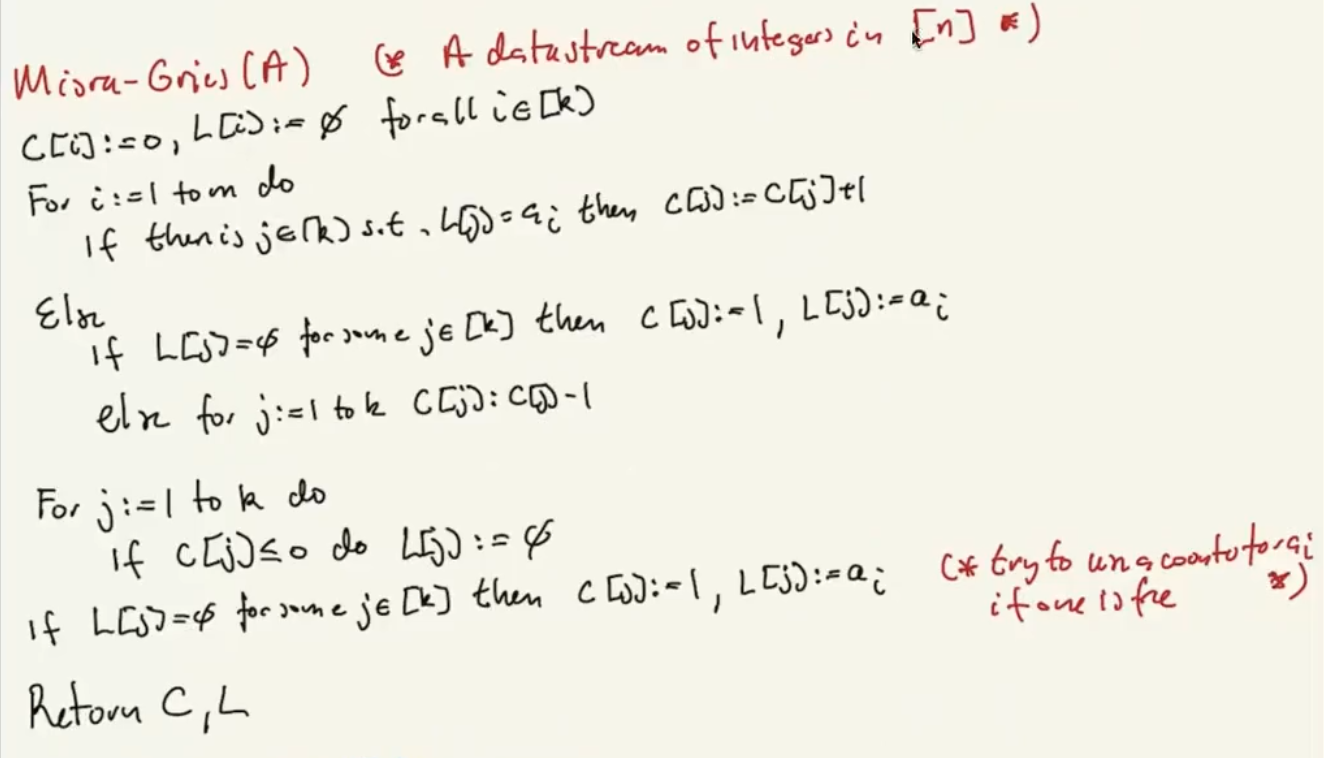
\includegraphics[scale=0.3]{misra.png}
\end{center}

Givet denne algoritme, hvis du giver en værdi $q \in [n]$, så,
\begin{itemize}
\item Hvis $\exists j \in [k]$ med $L[j]=q$, returnerer den $\hat{f}_q = C[j]$
\item Ellers returnerer $\hat{f}_{q} = 0$
\end{itemize}

\noindent
\large Korrekthed\\
\noindent
\begin{itemize}
\item En tæller $C[j]$ med $L[j] = q$ er kun incremented hvis $a_{i} = q$ så $f_{q} \leq f_{q}$ holder altid
\item Hvis $C[j]$ med $L[j] = q$ er decremtned, så er alle andre counters decremented
\end{itemize}


\subsection{Median-Finding og Quicksort}
\label{subsec:label}

Så for satan! Er vi klar?

Først, \texttt{Selec(S,k)}

MANGLER



\newpage

\section{Probabilistic Analysis}
\label{sec:proban}

\subsection{Coupon Collector}

Der er $n$ kuponner. Du kan få alle kuponnerne i morgenmadsprodukter. Givet at der er uniform sandsynlighed for hver kupon (dvs. $1/n$ sandsynlighed i hver karton), hvor mange kartoner kan du så forvente at åbne før du får alle $n$ kuponer?

Lad os starte med at introducere $X$ som er en random variable lig med antallet af bokse du skal købe indtil du har en kupon af hver type. Ydermere, lad os definere $X_{i} = \begin{cases}
  1 & \text{ hvis du får en kupon i kasse }i\\
  0 & \text{ ellers}
\end{cases}$

Dermed $X = X_{1}, X_{2}, \ldots, X_{n}$. Lad os finde den forventede værdi:

\begin{equation}
\begin{split}
  E[X] &= \sum_{j=0}^{n-1}E[X_{j}]\\
       &= \sum_{j=0}^{n-1} \frac{n}{n-j}\\
       &= n \sum_{j=0}^{n-1} \frac{1}{n-j} \\
       &= n \sum_{i=1}^{n} \frac{1}{i} \\
       &= nH(n) \\
  &= \Theta(n \log n)
\end{split}
\end{equation}

Dermed skal du forvente at købe $n \log n$ morgenmadsprodukter før du får alle $n$. 

\subsection{Forventede køretid af Quicksort og Selection}
\label{subsec:label}


\subsection{Randomiseret approximation for max $k$-SAT}
\label{subsec:label}

Dette bliver ``bare'' en generaliseret version af kapitel 13.3.

Givet et sæt af clauses, $C_{1}, \ldots, C_{j}}$, hvor af længde $k$, over et sæt af variabler $X = \{x_{1}, \ldots, x_{n}\}$, findes der en satisfying truth assignment?
Antag at vi sætter hver variabel $x_{1}, \ldots, x_{n}$ uafhængigt til 0 eller 1 med sandsynlighed $\frac{1}{2}$ hver. Hvad er det forventede antal af caluses satisfied?

Lad $Z$ være det random variable lig med antallet af satisfied clauses. Vi introducerer nu $Z_{i} = \begin{cases}
  1 & \text{ hvis clause }C_{i} \text{ er satisfied}\\
  0 & \text{ ellers}.
\end{cases}$

Dermed er $Z = Z_{1} + Z_{2} + \cdots + Z_{j}$. Givet at $E[Z_{i}]$ er sandsynligheden for at $C_{i}$ er satisfied, finder vi den hvis bare én af de $k$ literaler er 1. Sandsynligheden for dette \textbf{ikke sker} er $\left( \frac{1}{2} \right)^{k}$. Givet $k = 3$, så $\left( \frac{1}{2} \right)^{3} = \frac{1}{8}$

Dermed
\begin{equation}
\begin{split}
  E[Z] &=E[ \sum_{i=0}^{j} Z_{i} ]\\
       &= \sum_{i=0}^{j} 1-\left( \frac{1}{2} \right) ^{k}\\
  &= j 1-\left( \frac{1}{2} \right)^{k}
\end{split}
\end{equation}

\begin{theorem}
  \label{theorem:13.15}
For en $k-$SAT formel, hvor hver klausul har $k$ forskellige variabler, er det forventede antal af klausuler satisfied af en random assignemtn indenfor $(\frac{1}{2})^{k}$ af optimal.
\end{theorem}


\begin{theorem}
For hver instans af $k$-SAT er der en truth assignment der satisfier mindst en $\left 1-( \frac{1}{2} \right)^{k}$ del af alle klausuler.
\end{theorem}

Næste gælder udelukkende for $k = 3$. Hurtig recap: $1 - \left( \frac{1}{2} \right)^{3} = \frac{7}{8}$.

Vi argumenterer at hvis $j \leq 7$, altså, der er 7 eller færre klausuler, så er der et truth assignment der er satisfiable. Dette er fordi når $j \leq 7, $så $\frac{7}{8}j > j - 1$, og siden antallet af klausuler skal være et heltal, må det være lig med $j$.

\subsubsection{Ydere analyse}

Vi vil gerne have en randomiseret algoritme, hvis forventede køretid er polynomiel og den giver en sandhedstabel der satisfier mindst $\frac{7}{8}$ af alle klausuler.
Vi ved at dette kan findes, fra Teorem~\ref{theorem:13.15}. Men hvor lang tid kommer det til at tage, før vi finder en? 

Hvis vi kan finde sandsynligheden for at en tilfældig sandhedstabel satisfier mindst $\frac{7}{8}k$ klausuler er mindst $p$, så er den forventede antal af ``trials'' brugt af algoritmen $\frac{1}{p}$.
For $j = 0, 1, 2, 3\ldots, k$, lad $p_{j}$ være sandsynligheden for at en tilfældig truth assignment satisfier præcis $j$ klausuler. Så, det forventede antal af klausuler satisfied, gennem definitionen af forventning, er lig med \[
\sum_{j=0}^{k}j p_{j}
\]

Fra den tidligere analyse er dette lig $\frac{7}{8}k$.
Vi er interesserede i $p = \sum_{j \geq \frac{7}{8}k}^{}p_{j}$, altså, kun når der bliver satisfied mere end $\frac{7}{8}k$ klausuler.

Vi starter med at skrive:

\[
\frac{7}{8}k = \sum_{j=0}^{k}jp_{j} = \sum_{j < \frac{7}{8}k}^{} jp_{j} + \sum_{j \geq \frac{7}{8}k}^{} j p_{j}
\]

Nu definerer vi $k'$ til at være det største naturlige tal mindre end $\frac{7}{8}k$. Højresiden i ligningen bliver kun større hvis vi erstatter den første sum med $k'p_{j}$ og leddene i anden sum med $kp_{j}$. Ydermere observerer vi at $\sum_{j < \frac{7}{8}k}^{}p_{j} = 1 - p$ og så
\[
\frac{7}{8}k \leq \sum_{j < \frac{7}{8}k}^{} k'p_{j} + \sum_{j \geq \frac{7}{8}k}^{}kp_{j} = k'(1-p)+kp \leq k' + kp
\]

Og dermed er $kp \geq \frac{7}{8}k - k'$. Men $\frac{7}{8}k - k' \geq \frac{1}{8}$, siden k' er et heltal mindre end $\frac{7}{8}$ gange et andet heltal, så
\[
p \geq \frac{\frac{7}{8}k - k'}{k} \geq \frac{1}{8k}
\]


\label{subsec:label}



\newpage

\section{Indicator Random Variables}
\label{sec:indicator}

\section{Universal Hashing}
\label{sec:hashing}


I hashing har vi et univers der er meget større end størrelsen på tabellen hvortil hash funktionen finder et index. Dvs. $|U| >> m$, hvor $m$ er størrelsen på tabellen.

Problem med normal hashing: Der kan blive lavet angreb hvor en person der kender hash funktionens værdi kan lave en masse argumenter der alle hasher til det samme index. Vi fikser dette ved at tilfældigt og uafhængigt af nøglerne, vælge en universal hash funktion. På en universal hash funktion er sandsynligheden for at to værdier hasher til det samme $\leq 1/m$.

Vi kalder det en \textbf{kollision}, hvis to værdier hasher til den samme værdi. Vi ved naturligvis fra dueslagsprincippet (Teorem~\ref{theorem:pigeonhole}) at hvis der er mere end $m$ værdier der bliver hashet, så vil der være mindst én kollision. 


\subsection{Universal Hashing}

Lad $\mathcal{H}$ være en endelig kollektion af hash funktioner således at $h : U \rightarrow [m]$  for hver $h \in \mathcal{H}$.

\begin{theorem}
  Hash kollektionen $\mathcal{H}$ er \textbf{universal} hvis følgende holder:

  Lad $h \in \mathcal{H}$ være valgt tilfældigt. Så $\forall k, l \in U \text{ med } k \neq l \; \; p(h(k) = h(l)) \leq \frac{1}{m}$
  \end{theorem}

\begin{theorem}
  Antag at $h$ er valgt tilfældigt fra en universal kollektino $\mathcal{H}$ af hash funktioner fra $U \rightarrow [m]$.

  Antag at vi har brugt $h$ til at hashe et sæt $s \subseteq U$ med $|S| = n$ hvor vi bruger chaining til at løse kollisioner.

  Lad $T = T[0], T[1], \ldots, T[m-1]$ være tabellen af linked lister vi får når $T[i]$ er en linked list med de elementer $x \in S$ hvorfra $h(x) = i$.

  Derfra gælder følgende:
  \begin{itemize}
  \item Hvis $k \notin S$, så $E[n_{h(k)}] \leq \frac{n}{m} = \alpha$ hvor $n_{h(k)}$ er længden af $T[h(k)]$
  \item Hvis $k \in S$ så $E(n_{h(k)}) \leq \alpha + 1$
    \end{itemize}
 \end{theorem}

\begin{proof}
  $\forall k, l \in U, k \neq l$ definerer vi
  \[
    X_{kl} = \begin{cases}
      1 & \text{ hvis } h(k) = h(l) \\
      0 & \text{ hvis } h(k) \neq h(l) \\
      \end{cases}
  \]

  For et fixed $k \in U$ definerer vi $Y_{k} = |\{ l \in S \setminus \{k\} | h(k) = h(l) \}|$, altså er $Y_{k}$
  antallet af nøgler i $S \setminus \{k\}$ der hasher til samme værdi som $k$.

  Derfor ved vi at $Y_k = \sum_{l \neq k, l \in S} X_{kl}$


  \begin{equation}
    \begin{split}
      E(Y_{k}) &= E( \sum_{l \neq k, l \in S} X_{kl}) \\
               &= \sum_{l \neq k, l \in S} E(X_{kl}) \\
               &\leq \sum_{l \neq k, l \in S} \frac{1}{m}\\
    \end{split}
  \end{equation}

  \begin{itemize}
   \item Hvis $k \notin S$ så $n_{h(k)} = Y_{k}$  og $|\{l \in S | l \neq k\}| = |S| = n$ så \[ E(n_{h(k)}) = E(Y_{k}) \leq \sum_{l \neq k, l \in S} \frac{1}{m} = \frac{|S|}{m} = \frac{n}{m} = \alpha \]
   \item Hvis $k \in S$, så $n_{h(k)} = Y_{k}+1$ og $|\{l \in S | l \neq k\}| = |S|-1  = n - 1$ dermed \[ E(n_{h(k)}) = 1 + E(Y_{k}) \leq 1 + \sum_{l \neq k, l \in S} \frac{1}{m} = 1 + \frac{n-1}{m} \leq 1 + \alpha \]
  \end{itemize}
  
\end{proof}

\begin{corollary}
 Ved brug af Universal hashing + chaining, ved at starte fra en tom tabel med $m$ pladser, tager det forventet tid $O(n)$ til at lave en sekvens af \texttt{INSERT}, \texttt{SEARCH} og \texttt{DELETE} operations når $O(m)$ af dem er \texttt{INSERT}
\end{corollary}

\begin{proof}

  Vi indsætter $O(m)$ elementer, hvilket betyder at $|S| \in O(m)$. Dermed $\alpha = \frac{n}{m} \in O(1)$, fordi det er mindre end $m$.
  Den forventede længde af hver liste i tabellen er $O(1)$, så hver operation tager $O(1)$ forventede tid, så $O(n)$ for alle operationer. 
\end{proof}


\subsection{Design af Universal Class}

\subsubsection{Cormen}

Følgende er Cormen's metode til at lave en universal class:

\begin{itemize}
\item Vælg et primtal $p \geq |U|$ og antag at $U \subseteq \{0, 1, 2, \ldots, p-1\}$, $\mathbb{Z}_{p} = \{0,1,2, \ldots, p-1\}, \mathbb{Z}_{p}^{*} = \{1, 2, \ldots, p-1\}$
\item Fordi $p$ er et primtal kan vi løse ligninger $\mod p$.
\item $p \geq |U| > m$ så $p > m$.
\item For $a \in \mathbb{Z}_{p}^{*}$ og $b \in Z_{p}$ definér $h_{ab}(k) = ((ak+b) \mod p) \mod m$, $h_{ab} : \mathbb{Z}_{p} \rightarrow \mathbb{Z}_{m}$
\item Sæt $\mathcal{H} = \mathcal{H}_{pm} = \{h_{ab} | a \in \mathbb{Z}_{p}^{*}, b \in \mathbb{Z}_{p}\}$
\end{itemize}


\begin{theorem}
  Klassen $\mathcal{H}_{pm}$ er universal.
\end{theorem}


\subsubsection{KT}

I KT's metode identificerer vi universet $U$ med tupler af formen $(x_{1}, x_{2}, \ldots, x_{r})$ for et haltal når $0 \leq x_{i} < p$ for $i = 1, 2, \ldots, r$. Derudover antager vi at universet er $U \subseteq \{0, 1, 2, \ldots, N-1\}$. Antag ydermere at $n$ er størrelsen af hashtabellen, i den tidligere metode fra Cormen var dette $m$.

Da vi antager at universet er lavet af tal, kan vi konvertere de tal til binære tal á $log_{2}p$ bits. D.v.s, at hvis $p = 11$, og du har tallet $85$, som du gerne vil hashe. $log_{2}(11) = 3.45 \approx 4$. Vi tager 85 i binær: $1010101$. Længden af det binære tal er kun 7 ciffrer, derfor tager vi og tilføjer et 0 først (da dette ikke ændrer på tallet). Dermed bliver det $01010101$ som har 8 ciffrer. Vi kan dermed dele det op i 2, så vi har en vektor der hedder $(0101, 0101)$. Vi konverterer dette tilbage til heltal, $(5,5)$

 Hvor mange bits skal vi bruge til  at repreæsenterer et tal af størrelse $N$? $\log_{2}N$. Hvor mange stykker af længde $log_{2}P$ kan du lave? $\frac{\log_{2}N}{\log_{2}p} \approx r \approx \frac{\log N}{\log n}$. Det er stadig log 2, jeg er bare doven.

Lad $A = \{(a_{1}, a_{2}, \ldots, a_{r}) | a_{i} \in \{0, 1, 2, \ldots, p-1\} \forall i \in [r]\}$

For $a \in A$ lad
\[ h_{a}(x) = \left( \sum_{i=1}^{r} a_{i}x_{i} \right) \mod p \]

\[ \mathcal{H} = \{h_{a} | a \in A\} \]

\begin{theorem}
  $\mathcal{H}$ er en universal hashfamilie.
\end{theorem}

\begin{proof}
  Lad $x = (x_{1}, x_{2}, \ldots, x_{r})$ og $y = (y_{1}, y_{2}, \ldots, y_{r})$ være distinkte elementer fra $U$.

  Hvad vi nu vil vise er at når $a = (a_{1}, a_{2}, \ldots, a_{r}) \in A$ er valgt tilfældigt, så $p(h_{a}(x) = h_{a}(b)) \leq \frac{1}{p}$. Hvis det er højest $1/p$ er det også højest $1/n$, da $p > n$.

  Da $x \neq y$ er der et $j \in [r]$ således at $x_{j} \neq y_{j}$, altså, der \textbf{må} være en koordinat hvorpå de er uenige.

  Vi bruger følgende måde at vælge et tilfældigt $a \in A$ på:
  Først vælg alle $a_{i}, i \neq j$. Så vælg $a_{j}$. 


  Vi vil nu bevise at for hvert valg af $a_{i}$ hvor $i \neq j$, så er sandsynligheden for at det sidste valg af $a_{j}$ ender med $h_{a}(x) = h_{a}(y)$ er præcis $\frac{1}{p}$.

  \begin{equation}
\begin{split}
             h_{a}(x) &= h_{a}(y) \\
  \sum_{q=1}^{r}a_{q}x_{q} &= \sum_{q=1}^{r} a_{q}y_{q} \mod p \\
  \sum_{q = 1}^{r} a_{q}(x_{q}-y_{q}) &= 0 \mod p\\
  \sum_{q \neq j} a_{q} (x_{q} - y_{q}) + a_{j} (x_{j} - y_{j}) &= 0 \mod p \\
  \sum_{q \neq j} a_{q} (x_{q}-y_{q}) &= a_{j}(y_{j}-x_{j}) \mod p\\
  \end{split}
    \end{equation}

    Grunden til vi skriver $\mod p$ til sidst, er fordi, hvis $a \mod p = b \mod p$ så $a = b \mod p$.

    Efter vi har fikset $a_{i}$ for $i \neq j$ har vi $\sum_{q \neq j} a_{q}(x_{q} - y_{q}) = s \mod p$ for some $s \in \{0,1,2, \ldots, p-1\}$

    Dermed $h_{a}(x) = h_{a}(y)$ hvis og kun hvis $a_{j}(y_{j}-x_{j}) = s \ mod p$ da $z = y_{j} - x_{j} \neq 0$ siden vi har sikret os at $x_{j} \neq y_{j}$ har ligningen $a_{j}(y_{j}-x_{j}) = s \mod p$ en unik løsning $a_{j} = s (y_{j}-x_{j})^{-1} \mod p$
    Vi ved at $z$ ikke er 0, da vi antog at $i \neq j$.

    $a_{j}$ får en tilfældig værdi i $\{0, 1, 2, \ldots, p-1\}$ når $a = \{a_{1}, a_{2}, \ldots, a_{r}\}$ bliver konstrueret. Dermed er sandsynligheden at $a_{j} = s \cdot (y_{j} - x_{j})^{-1} \mod p$ holder (og dermed $h_{a}(x) = h_{a}(y)$) $1/p$. Q.E. FUCKING D.
\end{proof}

\subsection{Perfect Hashing}

Målet med Perfect Hashing er at få en virkelig god worst case behavior. Vi kan dog kun få det når nøglerne er statiske, så når tabellen er blevet lavet, kan nøglerne ikke ændres. Dette kan eksempelvis bruges i CD/DVD.

Vi ønsker at få $O(1)$ memory access i worst case (dvs. konstant tid selv i worst case), og et lavt memory use.

Perfect hashing bruger to niveauer af hashing hvor begge bruger universal hashing. Så først hashes der til tabel 1, og derefter hashes der til tabel 2, frem for en linked list. 
  
Ved level et finder vi et nøjagte valgt hash funktion $h \in \mathcal{H}$ når $h$ er universal.

I stedet for at bruge en linked list bruger vi en sekundær hashtabel $S_{j}$ sammen med en associeret hashfunktion $h_{j}$ for at undgå kollisioner i level 2. Størrelsen af $n_{j}$ vil være $n_{j}^{2}$ hvor $n_{j} = |\{x \in S | h(x) = j\}|$

Ved level 1 bruger vi $h \in \mathcal{H}_{pm}$ når $p > |S|\;\;(S \subseteq \{0, 1, 2, \ldots, p-1\})$ ( dette er familien af hash funktioner defineret fra Cormen)

Nøgler hvor $h(x) = j$ bliver hashet til tabellen $S_{j}$ af størrelsen $m_{j}$ ved brug af $h_{j} \in \mathcal{H}_{pm_{j}}$


Vores første mål er at vi skal blive sikre på at der er ingen collisions på level 2. Derefter skal vi vise at de forventede hukkommelsesbrug er $O(n), n = |S|$.

\begin{theorem}
  Antag at vi lagrer $n$ distinkte nøgler i en hashtabel af størrelse $m = n^{2}$ ved brug af en tilfældig $h \in \mathcal{H}$, når $\mathcal{H}$ er universal. Så er sandsynligheden at der er \textbf{ingen} kollisioner mindst $1/2$.
\end{theorem}

\begin{proof}

  Der er $\binom{n}{2}$ mulige kollisioner.
  Lad $Z_{kl} = \begin{cases} 1 &\text{hvis } h(k) = h(l) \\ 0 &\text{ellers} \end{cases}$

  Da $h$ er universal, gælder det at $p(Z_{kl} = 1) \leq \frac{1}{m} = \frac{1}{n^{2}}$ når $k \neq l$.

  Så $Z = \sum_{k, l \in S, k \neq l}^{}Z_{kl}$ er antallet af kollisioner.

  Vi bruger naturligvis vores elskede linearity of expectation til dette.
  \begin{equation}
    \begin{split}
      E(Z) &= E(\sum_{k, l \in S, l \neq s}^{}Z_{kl})\\
           &= \sum_{k,l \in S, k \neq l}^{} E(Z_{kl}) \\
           &\leq \sum_{k, l \in S, k \neq l}^{} \frac{1}{n^{2}}\\
           &= \frac{\binom{n}{2}}{n^{2}}\\
      &< \frac{1}{2}\\
    \end{split}
  \end{equation}

  Vi vil så gerne finde sandsynligheden for at antallet af kollisioner er større end 1. Det gør vi ved hjælp af \textbf{Markov's Inequality} (Teorem \ref{teorem:markovsinequality}):
  \[ p(Z \geq 1) \leq \frac{E(Z)}{1} = E(Z) < \frac{1}{2} \]

  Dermed er chancen for at der er 0 kollisioner større end $\frac{1}{2}$.
\end{proof}

Så, hvor mange gange skal vi køre algoritmen, før vi finder noget uden nogen kollisioner? I gennemsnit vil det være: $\frac{1}{p(Z=0)} < \frac{1}{\frac{1}{2}} = 2$

Vi møder dog et problem nu. \textbf{Hvad hvis $n$ er stort, og $n^{2}$ så er for stort?}. F.eks., hvis $n = 1000$, så er $n^{2} = 1 000 000$, og det er heller ikke usandsynligt at $n > 1 000 000$; så der kan du begynde at se nogle store problemer.

Vi \textbf{løser} dette problem ved at udelukkende bruge størrelsen at tabellen $n^2$ til andet niveau, og lade det første niveau være $n = m$.

Lad $h \in \mathcal{H}$ være hash funktionen vi bruger på level 1.

Lad $n_{j} = |\{x | h(x) = j\}|$\footnote{Altså, antallet af elementer der hasher til værdi $j$} og lad $S_{j}, j \in [m]$ være en tabel med $n_{j}^{2}$ entries og $h_{j}$ en kollisionsfri hash funktion der mapper fra $\{x | h(x) = j\}$ til $S_{j}$.

Ved level 1, når vi antager at $m = n$, altså, størrelsen af tabellen er lig $n$, så bruger vi $O(n)$ hukommelse til at lagre:
\begin{itemize}
\item Den primære hashtabel (da der er $n$ slots)
\item Tallene $m_{j} = n_{j}^{2}\;\;\;j \in [m]_{0}$
\item $a_{j} \in \mathbb{Z}_{p}^{*}, b_{j} \in \mathbb{Z}_{p}$ hvilke definerer det andet andet niveau af hash funktionen $n_{j}$ som bliver brugt når $\{x | h(x) = j\}$.
\end{itemize}

\begin{theorem}
Antag at vi lagrer $n$ nøgler i en hash funktion af størrelse $m = n$ ved brug af universal hashing, og lad $n_{j}, j \in \{0,1,2, \ldots, m\}$ være antallet af nøgler der bliver hashet til $j$ ($h(x) = j$). Så $E\left( \sum_{j=0}^{m-1}n_{j}^{2}  \right) < 2n$ ($n_{j}$ er en random variable der afhænger af valget af $h$)
\end{theorem}

\begin{proof}
  Husk at $\forall a \in \mathbb{Z}^{+}\;\;\; a + 2 \binom{a}{2} = a + a(a-1) = a^{2}$

  \begin{equation}
    \label{}
\begin{split}
  E \left( \sum_{j=0}^{m-1}n_{j}^{2} \right) &= E \left( \sum_{j=0}^{m-1} n_{j} + 2 \binom{n_{j}}{2} \right)\\
                                          &= E \left( \sum_{j=0}^{m-1}n_{j} \right) + 2E(\sum_{i=0}^{m-1}\binom{n_{j}}{2})\\
                                          &= E(n) + 2E(r)\\
  &= n + 2 E(r)\\
\end{split}
  \end{equation}

  Hvor $r$ er der totale antal kollisioner når vi bruger $h \in \mathcal{H}$, som altså er lig $\sum_{i=0}^{m-1}\binom{n_{j}}{2}$

  Fordi vi bruger universal hashing gælder det at $E(r) \leq \binom{n}{2} \cdot \frac{1}{m} = \binom{n}{2} \frac{1}{n} = \frac{n-1}{2}$
  Dermed \[ E \left( \sum_{j=0}^{m-1}n_{j}^{L} \right) \leq n + 2 \cdot \frac{n-1}{2} < 2n\]
\end{proof}

\begin{corollary}
  Hvis du vælger et hashing scheme således at $m = n$ på level et og $m_{j} = n_{j}^{2}\;\;j \in \{0,1, \ldots, n-1\}$ på level 2, så er det forvetenede plads brugt p åden sekundere hash tabel mindre end 2n. 
\end{corollary}

\begin{proof}
\[ E(\sum_{j=0}^{m-1}m_{j}) = E \left( \sum_{j=0}^{m-1}n_{j}^{2} \right) < 2n\]
\end{proof}

\begin{corollary}
Ved brug af at hashing scheme som det nævnt før, er sandsynligheden for at vi har brug for mere end $4n$ hukoemmelse i alt for det andet niveau af hash tabeller mindre end $\frac{1}{2}$.
\end{corollary}

\begin{proof}
  Vi Bruger markov's inequality:


  \begin{equation}
p \left( \sum_{j=0}^{m-1} m_{j} \geq 4n \right) \leq \frac{E \left( \sum_{j=0}^{m-1}m_{j} \right)}{4n} < \frac{2n}{4n} = \frac{1}{2}
  \end{equation}

\end{proof}

\subsubsection{Konklusion}

Ved at bruge få trials til at finde en god $h \in \mathcal{H}$ når $\mathcal{H}$ er universal, så kan vi hurtigt få et skema $(h \text{ ved niveau 1 }, h_{1}, h_{2}, \ldots, h_{m-1} \text{ ved niveau 2})$ som bruger en fin mængde hukommelse.


\subsection{Count-min Sketch}
\label{subsec:count-min-sketch}

Antag at $S$ er en datastrøm hvor vi vil estimere frekvenserne af elementerne som forekommer ofte i $S$, for eksempem til at løse heavy hitters.


\begin{itemize}
\item Lad $b,l$ være heltal.  
\item Lad $\mathcal{H}$ være en univerel familie af hash funktioner, $h \in \mathcal{H}$ hasher $U \rightarrow [b]$ når U er universet af alle mulige elementer i strømmen.
\item Lad $h_{1}, h_{2}, \ldots, h_{l}$ være dinstikte medlemmer fra $\mathcal{H}$
\item Når vi siger at $h_{i} \in \mathcal{H}$ er universal, mener vi at $h_{i}$ er et tilfældigt medlem af $\mathcal{H}$
\end{itemize} 

Vi bruger $h_{1}, h_{2}, \ldots, h_{l}$ til at bygge en $l \times b$ array $M$ af tællere som følger:

Til at starte med $M_{ij} = 0$ for $i \in [l]$ og $j \in [b]$.

For hvert element $x$ i datastrømmen, processer vi det som følger:
\begin{enumerate}
\item Vi går igennem hver række $l$, og så finder vi hash-værdien af $x$, $h_{l}(x)$, hvis den f.eks., er 6, så increaser vi tælleren ved første række, 6. kolonne med 1. 
\end{enumerate}

Count-min sketch finder et upper bound på frekvensen. Det er et upper-bound, fordi den muligvis tæller nogle andre tal med. 

Vi har set at $M_{i}, h_{i}(x)$\footnote{Hvor $M_{i}$ er række $i$ i tabellen} altid er mindst frekvensen af $x$ of ofte højere. Dette er fordi:
\begin{enumerate}
\item[(a)] Hver occurence af $x$ increaser $M_{i}, h_{i}(x)$ med en, så $M_{i}, h_{i}(x) \geq fx$ når $fx$ er den rigtige frekvens af $x$ indtil videre. 
\item[(b)] Hver occurence af a $y \neq x$ med $h_{i}(x) = h_{i}(y)$ wil også increase $M_{i}, h_{i}(x)$
\end{enumerate}


Lad $S_{n}$ være de første $n$ elementer i datastrømmen. Vi lader $f_{y}$ være frekvensen af $y$ i $S_{n}$. Vi lader $M_{i}, h_{i}(x)$ være $Z_{i,x}$. $Z_{i,x}$ er en random variable der afhænger af det tilfældige valg af $h_{i} \in \mathcal{H}$.
Vi definerer indicatoer random variable $I_{i,x}$ som følger:
\[
I_{i,x}(y) = \begin{cases}
  1 & \text{ hvis } h_{i}(x) = h_{i}(y)\\
  0 & \text{ ellers }\\
\end{cases}
\]

Da $h_{i}$ er en universal hash funktion er $p(I_{i,x}(y) = 1) \leq \frac{1}{b}$ hvor $b$ er størrelsen på hash tabellen.

Det følger fra (a) og (b) at:
\[
Z_{i,x} = f_{x} + \sum_{\{ y \in S_{n} | y \neq x \}}^{} f_{y} \cdot I_{i,x}(y) \geq f_{x}
\]

Hvad er så den forventede værdi af $Z_{i,x}$?

Vi kommer til at bruge $\sum_{y \in S_{n}}^{}f_{y}=n=|S_{n}|$

\begin{equation}
  \begin{split}
    E(Z_{i,x}) &= E(f_{x} + \sum_{\{ y \in S_{n} | y \neq x\}}^{}f_{y} \cdot I_{i,x}(y))\\
               &= E(f_{x}) + E(\sum_{\{y \in S_{n} | y \neq x\}}^{} f_{y} \cdot I_{i,x}(y))\\
               &= f_{x} + \sum_{\{ y \in S_{n} | y \neq x \}}^{} f_{y} \cdot E(I_{i,x}(y)) \\
               &\leq f_{x} + \sum_{\{y \in S_{n} | y \neq x\}}^{} f_{y} \cdot \frac{1}{b}\\
               &\leq f_{x} + \frac{1}{b} \sum_{\{y \in S_{n} | y \neq x\}}^{} f_{y}\\
               &\leq f_{x} + \frac{1}{b} \sum_{y \in S_{n}}^{} f_{y}\\
               &= f_{x} + \frac{n}{b}\\
  \end{split}
\end{equation}

Dermed er den forventede værdi ``off'' med \textbf{højest} $\frac{n}{b}$ (den forventede værdi!). Desværre, gennem dueslagsprincippet vil der være mange collisions, så længe $n > b$, hvilket den jo er.

Ved brug af Markov's Inequality vil vi nu gerne bounde sandsynligheden for at vores estimat for $f_{x}$ er mere end $\frac{2n}{b}$ væk.

\[
p(Z_{i,x}-f_{x} \geq \frac{2n}{b})  \leq \frac{E(Z_{i,x} - f_{x})}{\frac{2n}{b}} = \frac{\frac{n}{b}}{\frac{2n}{b}} = \frac{1}{2} 
\]

Så, sandsynligheden for at vores estimat er mere end $\frac{2n}{b}$ væk er $\frac{1}{2}$, hvilket, er en ret stort sandsynlighed.


Hvad så hvis vi kun kigger på den hash funktion der giver os det tætteste estimat? Lad $\hat{f_{x}} = \min_{i \in [l]} Z_{i,x}$, så $\hat{f_{x}} \geq f_{x}$ og siden $h_{1}, h_{2}, \ldots, h_{l}$ er uafhængige af hinanden betyder det at:
\[
p(\hat{f_{x}} - f_{x} \geq \frac{2n}{b}) \leq \frac{1}{2^{l}}
\]

Antag at vi er givet værdier $\varepsilon, \delta$ og vi vil finde
\[
p(\hat{f_{x}} - f_{x} \geq \varepsilon n) \leq \delta
\]

Vi ved fra den tidligere ligning at hvis vi tager $b = \frac{2}{\varepsilon}$ og $l = \log_{2} \left( \frac{1}{\delta} \right)$ så

\[
p(\hat{f_{x}} - f_{x} \geq \varepsilon n) = p(\hat{f_{x}} - f_{x} \geq \frac{2n}{b}) \leq 2^{-l} = 2^{-\log (\frac{1}{\delta})} = \frac{1}{\frac{1}{\delta}} = \delta
\]

Så $p(\hat{f_{x}} - f_{x} \geq \varepsilon n) \leq \delta$

Vi bruger $b \cdot l = \frac{2}{\varepsilon} \cdot \log \left( \frac{1}{\delta} \right)$ tællere til at implementere sketchen og så får vi akkuratheden $p(\hat{f_{x}} - f_{x} \geq \varepsilon n) \leq \delta$, uanset længden af datastrømmen.

\newpage

\section{String Matching}
\label{sec:string}

\subsection{Notation}
\label{subsec:stringnotation}

Jeg tænker ikke at der skal snakkes om det her til eksamen, men følgende er en liste af notation der er nødvendige for  forforståelse:

\begin{itemize}
\item \textbf{Strenge}: Arrays med karakterer (ligesom i programmeringssprog)
\item \textbf{Shift}: Hvor langt inde i en streng
\item $P[1..m]$: Mønster med længde $m$
\item $T[1..n]$: Tekst med længde $n$
\item $T[1..n-m]$: Den tekst vi leder efter. Vi er ikke interesseret i de sidste $m$, da de er længere end mønsterstrengen.
\item \textbf{P forekommer med shift s}: Du finder mønstret $s$ karakterer inde i teksten.
\item \textbf{Validt shift} et shift hvor mønsteret $P$ forekommer
\item \textbf{Invalidt shift} et shift hvor mønsteret $P$ \textbf{ikke} forekommer. 
\end{itemize}
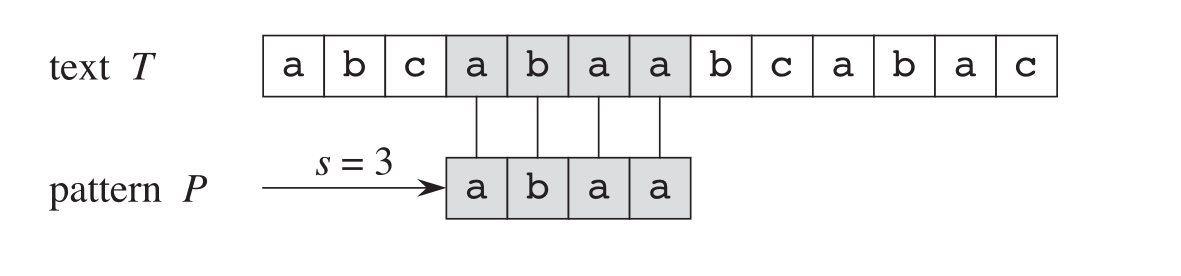
\includegraphics[width=400pt]{main--string-matching--notation-81a7.png}

\begin{itemize}
\item $\Sigma^{*}$ (Sigma-Stjerne) er sættet af alle endelige strenge der kan bliver lavet fra karaktererne i $\Sigma$. 
\item $\varepsilon$, den \textbf{tomme streng}, er strengen uden noget indhold. Den er også en del af $\Sigma^{*}$.
\item $|x|$ er længden af streng $x$. 
\item \textbf{Concatenation} af to strenge $x$ og $y$, skrevet $xy$ har længde $|x| + |y|$ og er karaktererne i $x$ efterfulgt af karaktererne i $y$.
\item \textbf{Præfiks} af streng $x$, denoted $w \sqsubset x$, gælder hvis $x = wy$ hvor $y \in \Sigma^{*}$, altså, $w$ er en del af streng $x$ i starten af strængen. $y$ er den resterende del af streng $x$, som ikke er $w$.
\item \textbf{Suffiks}: denoted $w \sqsupset x$ omvendt. 
\end{itemize}

\begin{lemma}[31.1 (Overlapping-suffix lemma) (Cormen)]
Suppose that $x,y$, and $z$ are strings such that $x \sqsupset z$ and $y \sqsupset z$. If $|x| \leq |y|$, then $x \sqsupset y$. If $|x| \geq |y|$, then $y \sqsupset x$. If $|x| = |y|$ then $x = y$.
\end{lemma}

\begin{proof}
  Se Figur ~\ref{fig:overlappingsuffix}
\end{proof}

\begin{figure}[ht]
  \centering
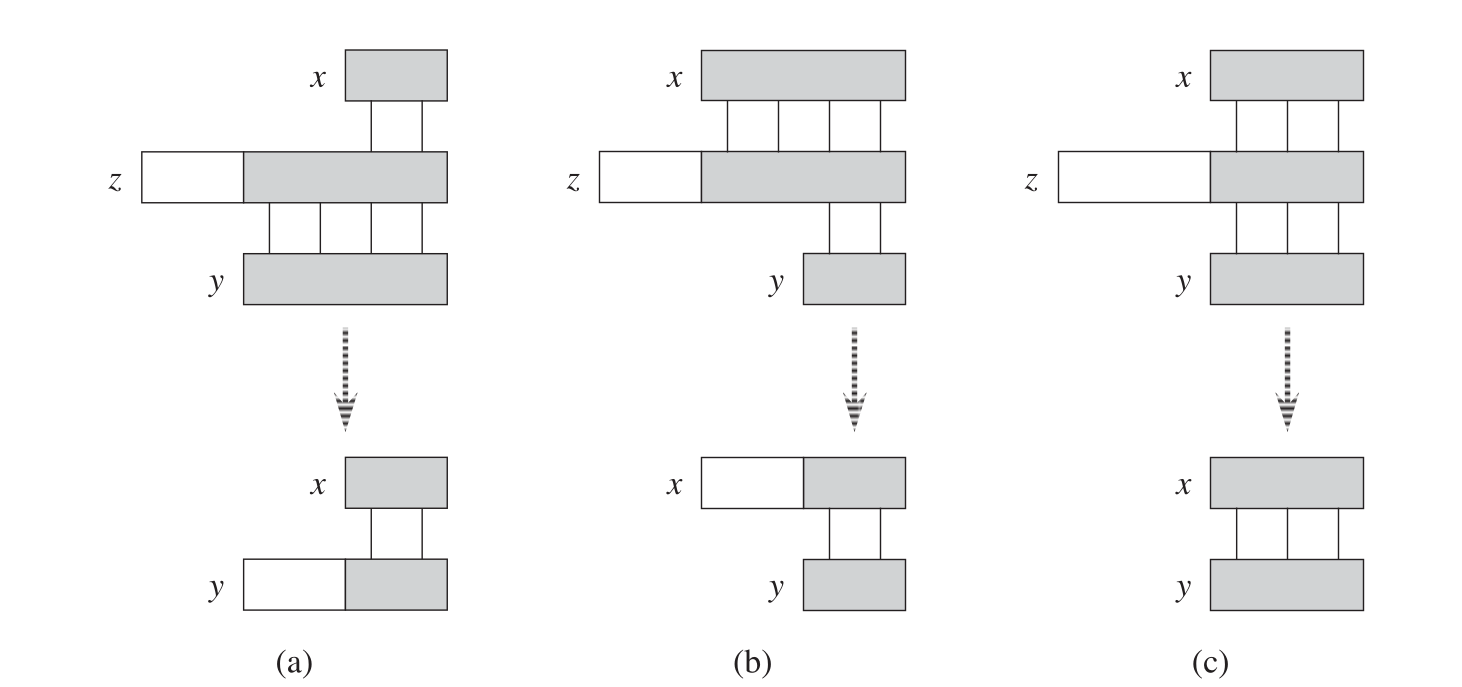
\includegraphics[width=400pt]{main--string-matching--notation-1e22.png}
  \caption{\label{fig:overlappingsuffix} Vi antager at $x \sqsupset z$ og $y \sqsupset z$. De tre dele af figuren illustrerer de tre cases af lemmaet. \textbf{(a)} Hvis $|x| \leq |y|$, så $x \sqsupset y$. \textbf{(b)} Hvis $|x| \geq |y|$, så $y \sqsupset x$. \textbf{(c)} Hvis $|x| = |y|$, så er $x = y$.}
\end{figure}

Vi antager at tiden det tager for at finde ligheden mellem to strenge er $\Theta(t+1)$ hvor $t$ er størrelsen af den længste streng. $+1$, til hvis $t = 0$.



\subsubsection{Køretids Overview}

\begin{table}[h]
\begin{tabular}{|l|l|l|}
\hline
\textbf{Algorithm}          & \textbf{Preprocessing Time} & \textbf{Matching Time} \\ \hline
\textit{Naive}              & $0$                         & $O((n-m+1)m)$          \\ \hline
\textit{Rabin-Karp}         & $\Theta (m)$                & $O((n-m+1)m)$          \\ \hline
\textit{Finite Automaton}   & $O(m |\Sigma |)$            & $\Theta (n) $          \\ \hline
\textit{Knuth-Morris-Pratt} & $\Theta (m)$                & $\Theta (n)$           \\ \hline
\end{tabular}
\end{table}


\subsection{Naive Algoritme}
\label{subsec:naive}

\begin{itemize}
\item Hvad er den? 
\item Hvorfor er den dårlig? 
\item Hvad er worst-case? 
\end{itemize}


Den naive algoritme er virkelig det, naiv.
\textbf{Source Code}:

\begin{verbatim}
Naive-String-Matcher(T,P)
n = T.length
m = P.length
for s = 0 to n - m
    if P[1..m] == T[s+1..s+m]
        print "Pattern occurs with shift " s
\end{verbatim}

\subsubsection{Køretid}

Den er virkelig skrald. Køretiden er $O((n-m+1)m)$. Dens worst case sker hvis teksten er $a^{n}$ og mønsteret der ledes efter er $a^{n}$ (begge er mængder af $a$'er, på længde hhv. $m$ og $n$. I dette tilfælde finder den matches hver gnag, og der tager dermed $O(n^{2})$ tid.

Der er \textbf{ingen} preprocessing tid, da der ikke skal gøres noget før algoritmen kører.



\subsection{Rabin-Karp}
\label{subsec:rabinkarp}

\begin{itemize}
\item Hvad er hovedidéen? 
\item Hvorfor er den bedre end naive? 
\end{itemize}

Trods at Rabin-Karp har en worst-case køretid på $\Theta((n-m+1)m)$ er dens gennemsnitlige køretid bedre.

Algoritmen konverterer bogstaverne til tal, i radix-$d$ notation, hvor $d$ er størrelsen på alfabetet, $|\Sigma|$.

I følgende eksempler vil vi gå ud fra at $d = 10$, og $\Sigma = \{0, 1, \ldots, 9\}$. Husk at $P[1..m]$ er mønsteret vi leder efter. Ved rabin-karp skelner vi mellem $P[1..m]$ og $p$, hvor $p$ er dets decimalværdi. Dvs., hvis $P[1..m] = 1372$, så er $p = 1372$ i decimalværdi. Eksemplet virker forsimplet idet vores alfabet også er tal, men tænk hvis alfabetet var $\Sigma = \{a, b, ... j\}$, i dette tilfælde ville $p$ ikke være ændret, men $P[1..m] = acgb$. Ydermere er teksten $T[1..n]$'s decimal counterpat $t_{s}$. Den bliver udregnet på samme måde. Hvis $t_{s} = p$ så $T[s+1..s+m] = P[1..m]$.

Vi vil gerne have en måde hvorpå vi kan lave alfabetet om til tal, som vi kan regne på. Hvis vi kan konverterer mønsteret $P[1..m]$ til $p$ på $\Theta(m)$ tid, så kan vi konvertere $t_{s}$ på $\Theta(n-m+1)$ tid. Til at gøre dette bruger vi \textbf{Horner's Rule}, som er meget vigtig at kende, se Definition ~\ref{def:horner}.

\begin{definition}[Horner's Rule]
  \label{def:horner}
  Horner's Rule er en regel hvorpå du hurtigt (specielt for computere) kan udregne decimaltal. Dette gør du ved at tage det sidste tal der skal udregnes først, derefter tager du tallet på 10'ernes plads, ganger det med $10^{1}$, etc. indtil du er ved $d$'ende plads, og ganger det med $10^{d}$\footnote{Dette gælder kun i base-10. Rabin-karp kører i base-b. Konverter dette til $b^{d}$}. Se følgende billede.


    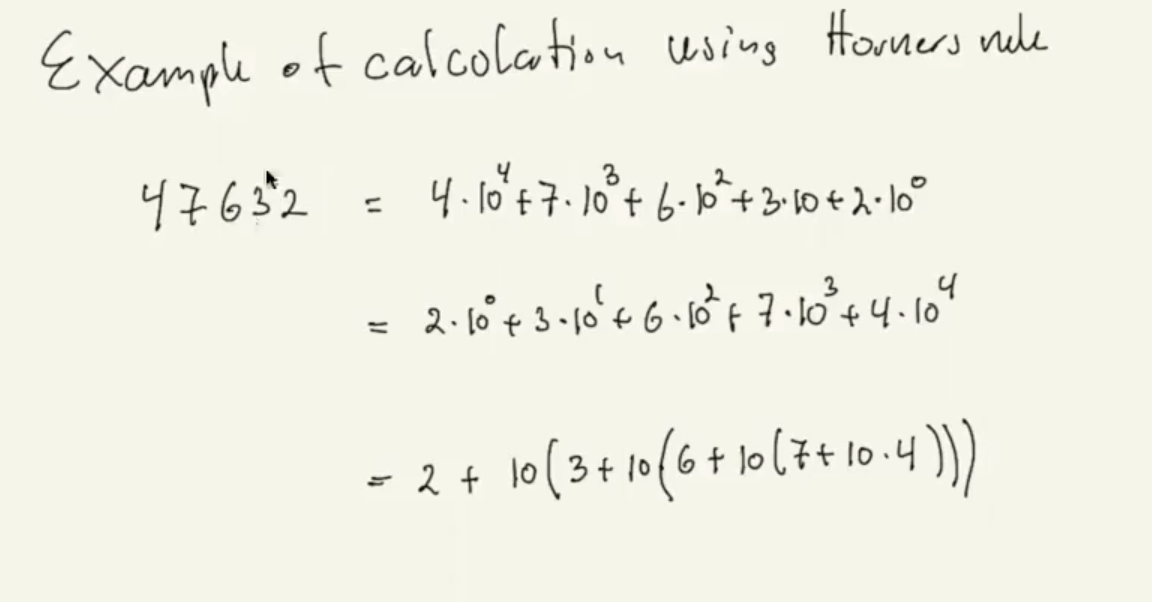
\includegraphics[width=300pt]{../Question8/main--the-naive-string-matching-algorithm--rabin-karp-c553.png} 
\end{definition}

Noget af det smarteste med Horner's Rule, er at, når du går til næste værdi, så kan du udregne det hurtigt uden at tage det hele om igen. Dette giver køretid $\Theta(n-m)$:

\[ t_{s+1} = 10(t_{s} - 10^{m-1}T[s+1]) + T[s+m+1] \]


\begin{forklaring}
\textit{Skip dette hvis du ikke har meget tid.} $10^{m-1} \cdot T[s+1]$ fjerner det højeste ciffer. Ved at gange det med 10 skifter du tallet til venstre med en cifferposition. Ved at tilføje $T[s+m+1]$ får du det nye, laveste ciffer. 
\end{forklaring}

\textbf{Problem!} $p$ og $t_{s}$ er muligvis for storre til at de kan være i et computer \texttt{word}. Hvis dette er tilfældet, og $P$ indeholder $m$ karakterer, så tager vi tallet \textbf{modulo }$q$. $p \mod q$ bliver udregnet på $\Theta(m)$ tid (størrelsen af $p$.) Alle $t_{s}$ værdier i $\Theta(n-m+1)$ tid.

\textbf{Hvilken $q$ skal vi dog vælge?} Simpelt! Vælg et primtal således der er plads til $10q$  i én computer \texttt{word}. Derefter kan vi udføre alle udregninger simpelt. Ved at bruge modulo-udregning, ændrer Horner's udregning sig til at blive: $t_{s+1} = (d(t_{s} - T[s+1]h) + T[s+m+1]) \mod q$, hvor $h \equiv d^{m-1} (\mod q)$ er værdien af ciffret $1$ i højeste position. 

\textbf{Problem igen!} Hvad hvis $p \equiv t_{s}$, men $P[1..m] \neq T[s+1..n-m]$? Altså, tallene er ens, men de er strengene ikke grundet modulo? Dette kalder vi et \textbf{spurious hit}, og er pisse irriterende, men desværre end nødvendig onde. Derfor, når vi finder et \textbf{hit} om det er spurious eller ej, så tjekker vi også strengene. 

\begin{figure}[ht]
  \centering
  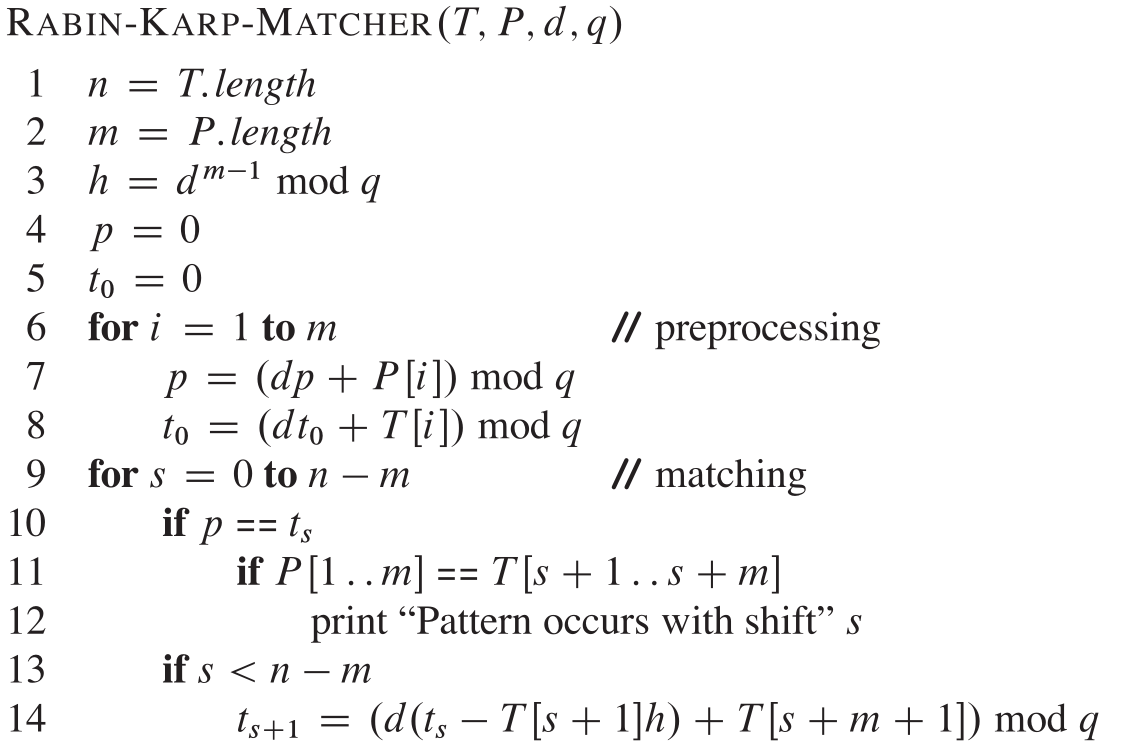
\includegraphics[width=400pt]{main--string-matching--rabin-karp-9fe7.png}
  \caption{\label{fig:rabinkarpalgorithm} Rabin Karp Algoritmen}
\end{figure}


Worst-case er i samme situation som ved den naive algoritme. Hvis teksten er en del a'er, og det samme med mønstret, så vil vi få en masse hits.



\subsubsection{Forventede antal hits}

Vi vil gerne finde det forventede antal hits. Vi antager at $\mod q$ agerer som en tilfældig mapping (funktion) fra alfabetet til heltal base $q$, altså $\Sigma^{*} \rightarrow \mathbb{Z}_{q}$. Ydermere antager vi at alle værdierne modulo $q$ er lige sandsynlige, i.e, $p(t_{s} \equiv p \mod q) = \frac{1}{q}$. Det vil sige at antallet af falske hits er $\frac{O(n)}{q} = O(\frac{n}{q}) $. Dette får vi fra antal af hvor mange der modulerer til samme værdi. Hvis der er 10 forskellige bogstaver, og vi er i base-3, så $\frac{10}{3} = 3.\overline{3}$ ca. tal der mapper til det samme.

Den forventede køretid bliver derfor $O(n) + O(m(v + \frac{n}{q}))$ hvor $v$ er antallet af korrekte hits, det's køretid er $O(1)$ og $q \geq m$. Dermed bliver den totale køretid $O(n+m) = O(n)$ da $n \geq m$.



\subsection{Finite Automaton Based}
\label{subsec:DFA}

\begin{itemize}
\item Hvordan laver man en DFA?
\end{itemize}

Jeg tænker \textbf{ikke} du behøver at forklare hvad en DFA er osv. Du får her en kort introduktion, som du bare kan springe over, givet at du forstår finite automata fint.

\subsection{Introduktion}
\label{subsec:DFAIntro}

Mange algoritmer bygger en Finite Automata (herfra forkortet som DFA), da den er utroligt hurtig til at finde matches. Hver karakter bliver kigget på præcis én gang, og bruger tid $O(1)$ per gang den bliver kigget på. Efter maskinen bliver bygget er matching tiden $\Theta(n)$. Dog kan tiden der bruges til at bygge maskinen være meget stor hvis $\Sigma$ er stort. 

\begin{definition}[Finite Automata]
  A \textbf{finite automaton} $M$, is a 5-tuple $(Q, q_{0}, A, \Sigma, \delta)$, where

  \begin{itemize}
  \item $Q$ is a finite set of \textbf{states}
  \item $q_{0} \in Q$ is the \textbf{start state}
  \item $A \subseteq Q$ is a disntinguished set of \textbf{accepting states},
  \item $\Sigma$ is a finite \textbf{input alphabet}, 
  \item $\delta$ is a function from $Q \times \Sigma$ into $Q$ called the \textbf{transition function} of  $M$.
  \end{itemize}
\end{definition}

Ved hvert state, læser maskinen et input, og går fra den state, $q$, til den næste defineret state, $\delta(q,a)$. Hvis $q$ er en del af $A$, og, efter strengen er blevet ``spist'', ender maskinen i $q \in A$, så er strengen ``accepteret'', ellers er den ikke. 

Ydermere bliver funktionen $\phi$ defineret som \textbf{Final-state funktion} fra $\Sigma^{*}$ til $Q$ således at $\phi(w)$ er den state som    $M$ ender op i, efter den scanner strengen $w$. Så, $M$ accepterer streng $w$ hvis \textbf{og kun hvis}, $\phi(w) \in A$.

\begin{equation}
  \label{eq:finalstatefunction}
\begin{split}
  \phi(\varepsilon) &= q_{0},\\
         \phi(wa) &= \delta(\phi(w),a) \; \; \text{for } w \in \Sigma^{*}, a \in \Sigma\\
\end{split}
\end{equation}


\subsection{Streng-matchende automat}
\label{subsec:stringmatchingautomata}


For at givet mønster $P$, vil vi lave en streng-matchende automat som preprocessing skridt før den bruges til at søge efter strengen.  Se figur~\ref{fig:stringmatchingautomata} for hvordan vi konsturerer automaten for mønstret $P = ababaca$. 

\begin{figure}[ht]
  \centering

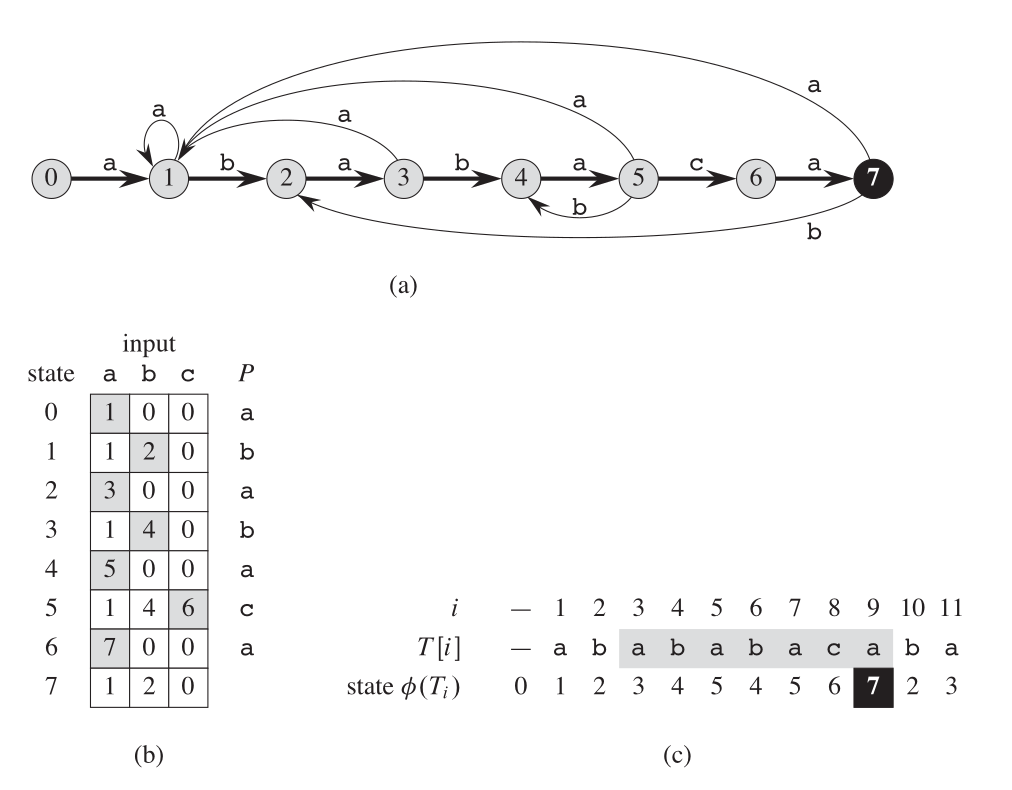
\includegraphics[width=400pt]{main--string-matching--streng-matchende-automat-6f23.png}  \caption{\label{fig:stringmatchingautomata} For mere information om figuren, se pp. 997 i Cormen}
\end{figure}


\begin{definition}[Suffiks Funktion]
  Givet et mønster $P[1..m]$, definerer vi funktionen $\sigma$, kaldet \textbf{suffiks funktion} korresponderende til $P$. Funktionen $\sigma$ mapper $\Sigma^{*}$ til $\{0,1, \ldots, m\}$, således at $\sigma(x)$ er længden af det længste præfix af $P$ som også er et suffiks af $x$:
  \[ \sigma(x) = \text{max}\{k : P_{k} \sqsupset x\} \]

  Suffiks Funktionen  er \textbf{well-defined} (hvert element mapper til noget), da $P_{0} = \varepsilon$ er et suffiks er hver streng. 
\end{definition}

\begin{example}[Eksempler på Suffiks Funktionen]

  Givet mønstret $P = ab$, har vi $\sigma(\varepsilon) = 0$, $\sigma(ccaca) = 1$ og $\sigma(ccab) = 2$.
  Givet mønstret med længde $m$ har vi $\sigma(x) = m$ hvis og kun hvis $P \sqsupset x$. Fra definitionen af suffiksfunktionen betyder $x \sqsupset y$ også at $\sigma(x) \leq \sigma(y)$.
\end{example}

Vi definerer en streng-matchende automat som korresponderende til et mønster $P[1..m]$ som følger:

\begin{itemize}
\item Sættet af states $Q$ er $\{0, 1, \ldots, m\}$. Start staten $q_{0}$, og staten $m$ er de eneste accepteret states. 
\item Transition function $\delta$ er defineret ved følgende ligning, for hver state $q$ og karakter $a$:

  \begin{equation}
    \label{32.4}
\delta(q,a) = \sigma(P_{q}a)
  \end{equation}
  
\end{itemize}

Det vil sige, at givet en karakter $a$, vil vi gå fra state $q$ til længden af det længste præfiks af $P$, som også er et suffiks af $x$. Så, altså, hvis $a$ får dig én længere, vil du også gå én state tilbage. Men, hvis du går tilbage til kun at være 2 inde, så er du tilbage på state 2. 

\begin{forklaring}[Yderligere forklaring]
  \label{forkl:yderligeredfa}
  Vi definerer $\delta(q,a) = \sigma(P_{q}a)$ fordi vi vil holde fast i det længste præfix af mønsteret $P$ der har matchet strengen $T$ indtil videre.

  Antag at $p = \phi (T_{i})$, så, efter at have læst $T_{i}$, så er automatonet i state $q$. Vi designer $\delta$ således at state $q$ fortæller os længden af det længste præfiks af $P$ der er en suffiks af $T_{i}$. Det vil sige, i state $q$, $P_{q} \sqsupset T_{i}$ og $q = \sigma(T_{i})$. Dette vil også sige at \textbf{hvis $q = m$, så har vi fundet et match!} Dermed, siden $\phi (T_{i})$ og $\sigma(T_{i})$ begge er lig $q$, ser vi at automaten holder følgende invariant:

  \begin{equation}
    \label{32.5}
\phi(T_{i}) = \sigma(T_{i})
  \end{equation}

  Dermed, hvis vi er i state $q$, og automaten læser karakter $T[i+1] = a$, så skal vores transition lede til det korresopnderende længste præfiks af $P$ som er et suffiks af $T_{i}a$. Den state er $\sigma(T_{i}a)$. 
  
Fordi $P_{q}$ er det længste præfiks af $P$ som er et suffiks af $T_{i}$, så er det længste præfiks af $P$ som er et suffiks af $T_{i}a$ ikke kun $\sigma(T_{i}a)$, men også $\delta(P_qa)$. (Dette bliver bevist senere)
\end{forklaring}

Der er to states vi skal kigge på, den første, $a = P[q+1]$, så er $\delta(q,a) = q+1$.
Den næste, $a \neq P[q+1]$, så skal vi finde et mindre præfiks af $P$ som også er et suffiks af $T_{i}$.

Lad os kigge på et eksempel. Streng-matching automaten fra Figur~\ref{fig:stringmatchingautomata} har $\delta(5,c) = 6$, som så er first case, hvor vi bare går videre. Et sekmepl på second case er $\delta(5, b) = 4$. Vi laver denne transition fordi, hvis automaten læser et $b$ når $q = 5$, så $P_{q}b = ababab$, og det længste præfiks af $P$ som også er et suffiks af $ababab$ er $P_{4} = abab$.

Følgende er algoritmen for at lave en finite automata til streng-matching. Sættet af states $Q = \{0, 1, \ldots, m\}$, start staten $q_{0} = 0$, den eneste accepting state er $m$, ${m} \in A$.


\begin{figure}[ht]
  \centering
  \begin{verbatim}
Finite-Automaton-Matcher(T, d, m):

n = T.length
q = 0
for i = 1 to n
    q = d(q, T[i])
    if q == m
        print "Pattern occurs with shift" i - m
\end{verbatim}
  \caption{\label{fig:dfa-algorithm} }
\end{figure}

Transition function er som beskrevet tidligere. Hvis dette ikke er klart, se Forklaring \ref{forkl:yderligeredfa}.

Det er her nemt at se at køretiden på en tekst-streng af længde $n$ er $\Theta(n)$.
Før vi viser pre-processing tid, kigger vi på et bevis for at algoritmen kører som forventet.


\begin{figure}[ht]
  \centering
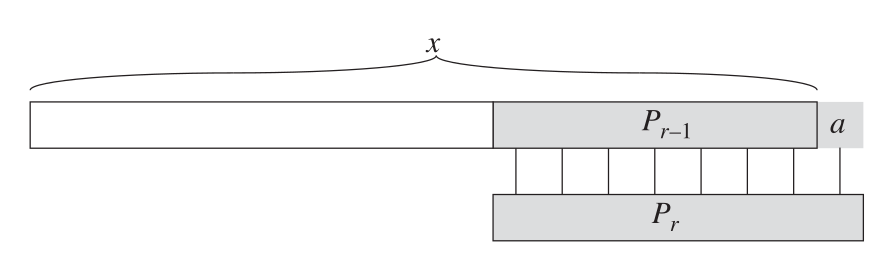
\includegraphics[width=300pt]{32.8.png}  
  \caption{\label{fig:32.8} En illustration til beviset af Lemma~\ref{lemma:suffixfunctioninequality}. FIguren viser $r \leq \delta(x) + 1$, hvor $r = \delta(xa)$}
\end{figure}


\begin{lemma}[Suffix-Function Inequality]
  \label{lemma:suffixfunctioninequality}
  For hver streng $x$ og karakter $a$, har vi at $\sigma(xa) \leq \sigma(x) + 1$.
\end{lemma}

\begin{proof}
Se Figur~\ref{fig:32.8}. Hvis $r = 0$, så $\sigma(xa) = r \leq \delta(x) + 1$ er trivielt løst, da $\sigma(x)$ er nonnegativt. Antag at $r > 0$, så $P_{r} \sqsupset xa$ per definition af $\sigma$. Dermed, $P_{r-1} \sqsupset x$, ved at fjerne $a$ fra enden af $P_{r}$ og fra enden af $xa$. Dermed $r-1 \leq \sigma(x)$, siden $\sigma(x)$ er det største $k$ således $P_{k} \sqsupset x$, og således $\sigma(xa) = r \leq \sigma(x) + 1$
\end{proof}

\begin{figure}[ht]
  \centering
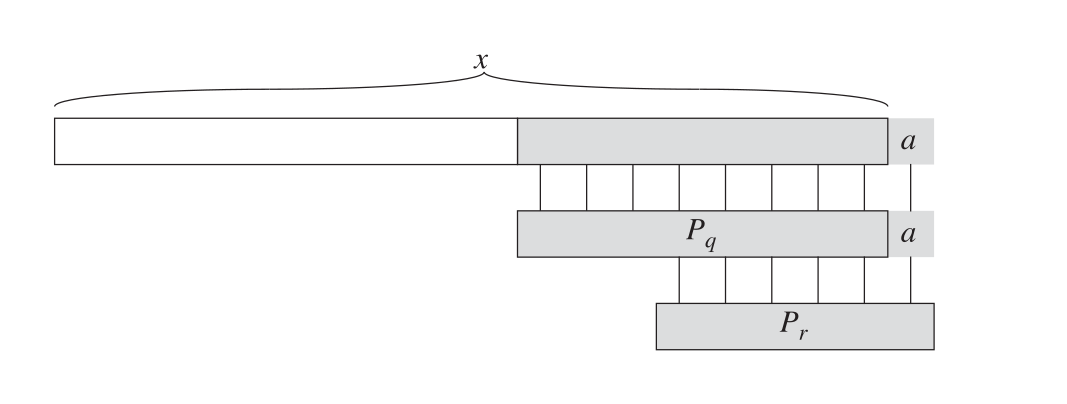
\includegraphics[width=300pt]{32.9.png}
  \caption{\label{fig:32.3} Illustration af beviset for Lemma~\ref{lemma:32.3}. Figuren fiser at $r = \delta(P_{q}a)$, hvor $q = \sigma(x)$ og $r = \sigma(xa)$}
\end{figure}


\begin{lemma}[Suffix-Function Recursion Lemma]
\label{lemma:32.3}
For enhver streng $x$ og karakter $a$, hvis $q = \sigma(x)$, så $\sigma(xa) = \sigma(P_{q}a)$.
\end{lemma}

\begin{proof}
Vi ved fra definitionen af $\sigma$ at $P_{q} \sqsupset x$. Som vist i figur~\ref{fig:32.3}, har vi også $P_{q}a \sqsupset xa$. Hvis $r = \sigma(xa)$, så $P_r \sqsupset xa$ og, gennem Lemma~\ref{lemma:suffixfunctioninequality}, $r \leq q + 1$. Dermed har vi at $|P_{r}| = r \leq q + 1 = |P_{q}a|$. Derfor, $r \leq \sigma(P_{q}a)$, dermed $\sigma(xa) \leq \sigma(P_qa)$. Vi har dog også $\sigma (P_{q}a) \leq \sigma(xa)$, siden $P_{q}a \sqsupset xa$. Dermed $\sigma(xa) = \sigma(P_{q}a)$
\end{proof}

Tid til det vigtigste skridt. Vi skal vise at automaten vedligeholder invarianten i ligning \ref{32.4}.

\begin{theorem}
  \label{the:32.4}
  If $\phi$ is the final-state function of a string-matching automaton for a given pattern $P$ and $T[1..n]$ is an input text for the automaton, then
  $\phi(T_{i}) = \sigma(T_{i})$
  for $i = 0, 1, \ldots, n$.
\end{theorem}

\begin{proof}
  Vi beviser gennem induktion på $i$.

 Ved $i = 0$ er teoremet sandt, da $T_{0} = \varepsilon$ dermed $\phi(T_{0}) = 0 = \sigma(T_{0})$.
\end{proof}

Vi antager nu at $\phi (T_{i}) = \sigma(T_{i}) $ og beviser at $\phi(T_{i+1}) = \sigma(T_{i+1})$.
Lad $q$ være $\phi(T_{i})$, og lad $a$ være $T[i+1]$.
Så:

\begin{equation*}
  \begin{split}
    \phi(T_{i+1}) &= \phi T(_{i}) \; \text{(fra definition på } T_{i+1}  \text{ og } \text{a})\\
               &= \delta(\phi (T_{i}), a) \; \text{(fra definitionen på} \phi \text{)}\\
               &= \delta(q,a) \; \text{(af defintiion på q)}\\
               &= \sigma(P_{q}a) \; \text{(fra definitionen tidligere)}\\
               &= \sigma(T_{i}a)\\
               &= \sigma(T_{i+1})\\
  \end{split}
\end{equation*}


\subsection{Find Transition Function}

Vi vil gerne finde transition funktion. Vi har allerede defineret den tidligere, men vi vil have en algoritmisk metode hvorpå vi kan gøre det.


\begin{figure}[ht]
  \centering
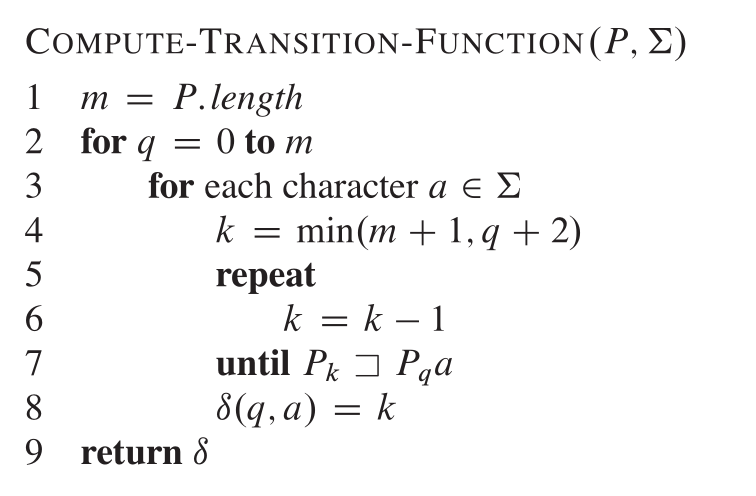
\includegraphics[width=250pt]{compute-transition-function.png}
  \caption{\label{fig:compute-transition-function} Algoritmen for at finde transition function på.}
\end{figure}

Køretiden på algoritmen er $O(m^{3}|\Sigma|)$.


\newpage


\section{Flows}
\label{sec:flows}

Et \textbf{netværk} $N = (V,E,C)$ er en digraph med en associeret funktion, kapacitetsfunktionen $c : E \rightarrow \mathbb{R}_{0}$ ($c(u,v) \geq 0 \forall (u,v) \in A$). I et netværk, hvis $(u,v) \notin E$, så $c(u,v) = 0$.
Ydermere er der en assumption i Cormen, om at parallele grafer ikke er tilladt, altså, hvis $(u,v) \in E,$ så $(v,u) \notin E$.

Jørgen's definition af flow er mere generel end den i Cormen:

\begin{theorem}[Flow]
  Et \textbf{flow} $f$ i $N$ er en funktion $f : E \rightarrow \mathbb{R}_{0}$ således at $0 \leq f(u,v) \leq c(u,v) \forall (u,v) \in E$
\end{theorem}

\begin{theorem}[Balance]
  \textbf{Balancen}  $b_{f}$ af et flow $f$ er funktionen
  \[
    b_{f}(v) = \sum_{(v,w) \in E}^{} f(v,w) - \sum_{(u,v) \in E}^{} f(u,v)
  \]
\end{theorem}

Altså, \textbf{balancen} af et flow er mængden af flow der kommer ud af en knude ($v$) minus mængden af flow der kommer ind. 


Vi kan her lave den observation at, hvis vi summerer alle balancer i flows, må deres sum blive 0, i.e., $\sum_{v \in V}^{} b_{f}(v) = 0$.

\begin{proof}
  $b_{f}(v) = \sum_{(v,w) \in E}^{}f(v,w) - \sum_{(u,v) \in E}^{}f(u,v)$
  så i $\sum_{v \in V}^{}b_{f}(v)$ bidrager hver kant $(u,v)$ med $f(u,v)$, og $b_{f}(v)$ og, $-f(u,v)$ i $b_{f}(u)$ så 0 i alt.
\end{proof}

\begin{definition}
  Lad $N = (V,E,c)$  være et netværk, og lad $s, t \in V$ være distinkte punkter. Et flow $f$ i $N$ er et $(s,t)-$flow, hvis der er et $K \geq 0$ således at
  \[
    b_{f}(v) =
    \begin{cases}
      k & \text{ hvis } v = s \\
      -k & \text{ hvis } v = t\\
      0 & \text{ hvis } v \notin \{s, t\}
    \end{cases}
    \]
\end{definition}

Altså, \textit{source} knuden har balance lig med flow, da der ikke kommer noget ind, og \textit{sink} knuden har balance lig med minus flow, da intet kommer ud. Dette gælder fordi et $(s,t)-$flow overholder \textbf{flow conservation}, hvilket vil sige at hvad der kommer ind, må også komme ud, og omvendt. 

\begin{definition}
  Værdien af et $(s,t)$-flow $f$ i $N = (V,E,c)$ er skrevet $|f|$ og er defineret til at være
  \[
|f| = \sum_{u \in V}^{}f(s,v) - \sum_{v \in V}^{} f(v,s)
  \]
\end{definition}

Altså, alt det flow der kommer ud fra source knuden, versus det der kommer ind.  Dermed er det det samme som $b_{f}(s)$, og $-b_{f}(t)$.

\begin{definition}
  Maksimum-flows problemet på et netværk $N = (V,E,c)$ med $s,t$ skal man maksimere $K$ således at

  \[
b_{f}(v) = \begin{cases}
  k & \text{ hvis } v = s\\
  -k & \text{ hvis } v = t\\
  0 & \text{ hvis } v \notin \{s,t\}\\
\end{cases}
    \]

    \[
0 \leq f(u,v) \leq c(u,v) \;\;\;\; \forall (u,v)
    \]
\end{definition}

Jørgen skelner mellem \textbf{maximum} og \textbf{maksimalt} flow. Et maksimalt flow kan ikke increases længere, \textbf{men} det er ikke maximum! Et maximumsflow er der ingen måder hvorpå værdien af $(s,t)-$flowet kan blive større.

Vi er nu efterladt med to spørgsmål:
\begin{itemize}
\item Hvordan ved vi at et flow er maximum?
\item Hvordan finder vi et flow der er maximum?
\end{itemize}

\noindent
{\Large \textbf{Cuts}}
\noindent

\begin{definition}
Lad $N = (V,E,c)$ være et netværk med source $s$ og sink $t$. Et $(s,t)-$cut er en partition $V = S \cup T$ hvor $T = V \setminus s$ og $s \in S, t \in T$. Kapaciteten af $(s,t)-$cut $(S,T)$ er $c(S,T) = \sum_{u \in S, v \in T}^{}c(u,v)$
\end{definition}

\begin{lemma}
  Lad $N = (V,E,c)$ være et netværk og $f$ et $(S,T)$-flow i $N$. Så, for hvert $(s,t)$-cut $(S,T)$ i $N$, har vi at:
  \[ |f| = f(S,T) - f(T,S) \]
\end{lemma}

\begin{proof}
\begin{equation}
  \begin{split}
    |f| &= \sum_{v \in S}^{} b_{f}(v)\\
        &= \sum_{v \in S}^{} \left(  \sum_{(v,w) \in E}^{} f(v,w) - \sum_{(u,v) \in E}^{} f(u,v) \right)\\
        &= \sum_{v \in S} \sum_{w \in T} f(v,w) - \sum_{u \in T, v \in S}^{}f(u,v) = f(S,T) - f(T,S)\\
  \end{split}
\end{equation}
\end{proof}

\begin{lemma}
  For hvert $(s,t)$-cut $(S,T)$ i $N = (V,E,c)$ og hvert $(s,t)$-flow $f$ i $N$, har vi at
  \[
|f| \leq c(S,T)
  \]
\end{lemma}

\begin{proof}
\begin{equation*}
  \begin{split}
    |f| &= f(S,T) - f(T,S)\\
    &\leq c(S,T) - 0 \;\;\;\; \text{ da } f(u,v) \leq c(u,v) og f(u,v) \geq 0\\
    &= c(S,T)
  \end{split}
\end{equation*}
\end{proof}

\subsection{Residual Networks}
\label{subsec:residual}

Lad $N = (V,E,c)$ og lad $f$ være et $(s,t)-$flow i $N$. \textbf{Residual Netværket} $N_{f}$ af $N$ med respekt til $f$ er $N_{f} = (V, E_f, c_{f})$, når

\[
c_{f}(u,v) = \begin{cases}
  c(u,v) - f(u,v) & \text{ hvis } (u,v) \in E\\
  f(u,v) & \text{ hvis }(v,u) \in E\\
  0 & \text{ ellers}
\end{cases}
\]
\textbf{Husk} at vi antager ingen anti-parallele kanter. 
Ydermere er $E_{f} = \{(u,v) \in V \times V | c_{f}(u,v) > 0\}$, altså, kanterne i residualnetværket er kanter hvis residual kapacitet er større end 0.

\textbf{Hvad skal vi bruge et residualnetværk til?} Simpelt! Vi bruger det til at finde vejene til et maximum flow.


Hver direkted $(s,t)$-path (vej) i $N_{f}$ korresponderer til en vej i $N$. 
Lad
\begin{equation}
  \begin{split}
  \delta_{-}(p) &= \min \{c(u,v) - f(u,v) | (u,v) \text{ er fremadgående på } P'\}\\
  \delta_{+}(p) &= \min\{ f(u,v) | (u,v) \text{ er tilbagegående på } P'\}\\
  \delta(p) &= \min\{ \delta_{+}(p), \delta_{-}(p)\}
  \end{split}
\end{equation}

Dette resultat er skrevet $(f \uparrow f_{p})$, og er et $(s,t)$ flow af værdi $|f| + |f_{p}| = |f| + \delta(p)$

Hovedidéen er simpel:
\begin{itemize}
\item $0 \leq (f \uparrow f_{p})(u,v) \leq c(u,v) $ af definitionen på $\delta(p)$
\item $(f \uparrow f_{p}) $ er et $(s,t)-$flow siden we tilføjer det samme mængde flow i hver $v \neq s,t$ som ud af det. 
\item $|f \uparrow f_{p}| = |f| + |f_{p}| = |f| + \delta(p)$ da vi increase flowet med $\delta(p)$ på præcis en ud af s.
\end{itemize}

Vi kalder en directed $(s,t)$-vej $P$ i $N_{f}$ en \textbf{augmenting path} og dens kapacitet er værdien $\delta(p)$ som vi udregnede. 

\subsection{Ford-Fulkerson}
\label{subsec:fordfulkerson}

Ford-fulkerson er en metode (ikke algoritme, da den mangler noget for implementation) til at finde maximum flow. Den tager som input et netværk hvor kapacitetsfunktionen $c$ udelukkende bruger heltal, og $s \neq t$. Dens output er et maximum $(s,t)$ flow $f$ i $N$.

\begin{center}
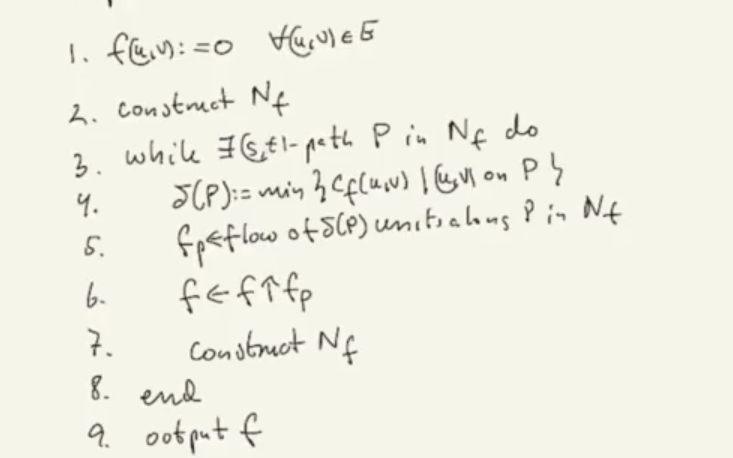
\includegraphics[scale=0.5]{ff.png}
\end{center}

Husk at så længe $N_{f}$ har et augmenting path $P$, så ved vi at $f$ ikke er maksimum, da $|f \uparrow f_{p}| = |f| + |\delta(p)| > |f|$.
Siden vi udelukkende dealer i integers, gælder det førsagte, da vi altid increaser med mindst én. Derfor findes der også et max-flow med sikkerhed. Dette bliver udvidet i følgende teorem:

\begin{theorem}[Max-flow Min-Cut]
  Hvis én af disse gælder, gælder alle:
  \begin{enumerate}
  \item[(1)]\label{item:1} $f$ er et maximum flow
  \item[(2)]\label{item:2} Der er ingen $(s,t)$-path i $N_{f}$
  \item[(3)]\label{item:3}  $|f| = c(S,T)$ for et $(s,t)$-cut $(S,T)$
  \end{enumerate}
\end{theorem}

37:15




\section{Min-Cut}
\label{sec:mincut}

\section{Misc}
\label{sec:misc}


Nået til 15:15 i video









\end{document}
